%%% Hlavní soubor. Zde se definují základní parametry a odkazuje se na ostatní části. %%%

%% Verze pro jednostranný tisk:
% Okraje: levý 40mm, pravý 25mm, horní a dolní 25mm
% (ale pozor, LaTeX si sám přidává 1in)
\documentclass[12pt,a4paper]{report}
\setlength\textwidth{145mm}
\setlength\textheight{247mm}
\setlength\oddsidemargin{15mm}
\setlength\evensidemargin{15mm}
\setlength\topmargin{0mm}
\setlength\headsep{0mm}
\setlength\headheight{0mm}
% \openright zařídí, aby následující text začínal na pravé straně knihy
\let\openright=\clearpage

%% Pokud tiskneme oboustranně:
% \documentclass[12pt,a4paper,twoside,openright]{report}
% \setlength\textwidth{145mm}
% \setlength\textheight{247mm}
% \setlength\oddsidemargin{14.2mm}
% \setlength\evensidemargin{0mm}
% \setlength\topmargin{0mm}
% \setlength\headsep{0mm}
% \setlength\headheight{0mm}
% \let\openright=\cleardoublepage

%% Vytváříme PDF/A-2u
\usepackage[a-2u]{pdfx}

%% Přepneme na českou sazbu a fonty Latin Modern
\usepackage[czech]{babel}
\usepackage{lmodern}
\usepackage[T1]{fontenc}
\usepackage{textcomp}

%% Použité kódování znaků: obvykle latin2, cp1250 nebo utf8:
\usepackage[utf8]{inputenc}

%%% Další užitečné balíčky (jsou součástí běžných distribucí LaTeXu)
\usepackage{amsmath}        % rozšíření pro sazbu matematiky
\usepackage{amsfonts}       % matematické fonty
\usepackage{amsthm}         % sazba vět, definic apod.
\usepackage{bbding}         % balíček s nejrůznějšími symboly
			    % (čtverečky, hvězdičky, tužtičky, nůžtičky, ...)
\usepackage{bm}             % tučné symboly (příkaz \bm)
\usepackage{graphicx}       % vkládání obrázků
\usepackage{fancyvrb}       % vylepšené prostředí pro strojové písmo
\usepackage{indentfirst}    % zavede odsazení 1. odstavce kapitoly
\usepackage{natbib}         % zajištuje možnost odkazovat na literaturu
			    % stylem AUTOR (ROK), resp. AUTOR [ČÍSLO]
\usepackage[nottoc]{tocbibind} % zajistí přidání seznamu literatury,
                            % obrázků a tabulek do obsahu
\usepackage{icomma}         % inteligetní čárka v matematickém módu
\usepackage{dcolumn}        % lepší zarovnání sloupců v tabulkách
\usepackage{booktabs}       % lepší vodorovné linky v tabulkách
\usepackage{paralist}       % lepší enumerate a itemize
\usepackage{xcolor}         % barevná sazba

%%% Údaje o práci

% Název práce v jazyce práce (přesně podle zadání)
\def\NazevPrace{Vizuální browser grafových dat}

% Název práce v angličtině
\def\NazevPraceEN{Visual browser of graph data}

% Jméno autora
\def\AutorPrace{Štěpán Stenchlák}

% Rok odevzdání
\def\RokOdevzdani{2020}

% Název katedry nebo ústavu, kde byla práce oficiálně zadána
% (dle Organizační struktury MFF UK, případně plný název pracoviště mimo MFF)
\def\Katedra{Katedra softwarového inženýrství}
\def\KatedraEN{Department of Software Engineering}

% Jedná se o katedru (department) nebo o ústav (institute)?
\def\TypPracoviste{Katedra}
\def\TypPracovisteEN{Department}

% Vedoucí práce: Jméno a příjmení s~tituly
\def\Vedouci{doc. Mgr. Martin Nečaský, Ph.D.}

% Pracoviště vedoucího (opět dle Organizační struktury MFF)
\def\KatedraVedouciho{Katedra softwarového inženýrství}
\def\KatedraVedoucihoEN{Department of Software Engineering}

% Studijní program a obor
\def\StudijniProgram{Informatika}
\def\StudijniObor{Softwarové a datové inženýrství}

% Nepovinné poděkování (vedoucímu práce, konzultantovi, tomu, kdo
% zapůjčil software, literaturu apod.)
\def\Podekovani{%
Chtěl bych poděkovat svému vedoucímu doc. Mgr. Martinovi Nečaskému, Ph.D. za jeho čas a pomoc, kterou mi poskytl při vypracování této práce. Současně mu děkuji za pomoc s výběrem tohoto tématu, které mě bavilo řešit. Dále děkuji své rodině, která mi umožnila v klidu práci dokončit.
}

% Abstrakt (doporučený rozsah cca 80-200 slov; nejedná se o zadání práce)
\def\Abstrakt{%
Jedním ze způsobů, jak publikovat data ve strojově čitelné podobě na internetu, je formou grafu. Taková data je pak velmi snadné propojovat mezi různými datovými zdroji a vytvořit tak velkou síť propojených dat. Abychom tyto data mohli vizualizovat, musíme používat nástroje na procházení grafu, které mohou být často nepraktické, neboť nám obvykle zobrazí veškeré informace, kterých mohou být stovky.

Cílem této práce je vytvořit webovou aplikaci, která je schopna tyto grafová data vizualizovat, poskytovat k nim informace a procházet je pomocí takzvaných konfigurací. Konfigurace popisuje, jaké data z velké množiny dat na internetu chceme zobrazit, jak je vizualizujeme a jak se na ně můžeme dívat. Dovolí nám tedy odfiltrovat stovky nezajímavých informací a odstíní tak uživatele od složité sítě propojených dat, aby se mohl věnovat pouze těm, která ho zajímají.
}
\def\AbstraktEN{%
One way to publish data in a machine-readable form on the Internet is in the form of a graph. Such data are easy to interconnect between different data sources and thus create a large network of linked data. In order to visualize this data, we need to use graph tools, which can often be impractical because they usually show us all the information about the graph.

The aim of this work is to create a web application that is able to visualize those graph data, provide information about them, and browse them using so-called configurations. The configuration describes what data from a large set of data on the Internet we want to display, how we visualize them, and how we can look at them. It allows us to filter out hundreds of uninteresting information, thus shielding users from a complex network of linked data so that users can focus on the data that interests them.
}

% 3 až 5 klíčových slov (doporučeno), každé uzavřeno ve složených závorkách
\def\KlicovaSlova{%
{RDF} {databáze} {graf} {linked data} {webová aplikace}
}
\def\KlicovaSlovaEN{%
{RDF} {database} {graph} {linked data} {web application}
}

%% Balíček hyperref, kterým jdou vyrábět klikací odkazy v PDF,
%% ale hlavně ho používáme k uložení metadat do PDF (včetně obsahu).
%% Většinu nastavítek přednastaví balíček pdfx.
\hypersetup{unicode}
\hypersetup{breaklinks=true}

%% Definice různých užitečných maker (viz popis uvnitř souboru)
%%% Tento soubor obsahuje definice různých užitečných maker a prostředí %%%
%%% Další makra připisujte sem, ať nepřekáží v ostatních souborech.     %%%

%%% Drobné úpravy stylu

% Tato makra přesvědčují mírně ošklivým trikem LaTeX, aby hlavičky kapitol
% sázel příčetněji a nevynechával nad nimi spoustu místa. Směle ignorujte.
\makeatletter
\def\@makechapterhead#1{
  {\parindent \z@ \raggedright \normalfont
   \Huge\bfseries \thechapter. #1
   \par\nobreak
   \vskip 20\p@
}}
\def\@makeschapterhead#1{
  {\parindent \z@ \raggedright \normalfont
   \Huge\bfseries #1
   \par\nobreak
   \vskip 20\p@
}}
\makeatother

% Toto makro definuje kapitolu, která není očíslovaná, ale je uvedena v obsahu.
\def\chapwithtoc#1{
\chapter*{#1}
\addcontentsline{toc}{chapter}{#1}
}

% Trochu volnější nastavení dělení slov, než je default.
\lefthyphenmin=2
\righthyphenmin=2

% Zapne černé "slimáky" na koncích řádků, které přetekly, abychom si
% jich lépe všimli.
\overfullrule=1mm

%%% Makra pro definice, věty, tvrzení, příklady, ... (vyžaduje baliček amsthm)

\theoremstyle{plain}
\newtheorem{veta}{Věta}
\newtheorem{lemma}[veta]{Lemma}
\newtheorem{tvrz}[veta]{Tvrzení}

\theoremstyle{plain}
\newtheorem{definice}{Definice}

\theoremstyle{definition}
\newtheorem*{dusl}{Důsledek}
\newtheorem*{pozn}{Poznámka}
\newtheorem*{prikl}{Příklad}

%%% Prostředí pro důkazy

\newenvironment{dukaz}{
  \par\medskip\noindent
  \textit{Důkaz}.
}{
\newline
\rightline{$\qedsymbol$}
}

%%% Prostředí pro sazbu kódu, případně vstupu/výstupu počítačových
%%% programů. (Vyžaduje balíček fancyvrb -- fancy verbatim.)

\DefineVerbatimEnvironment{code}{Verbatim}{fontsize=\small, frame=single}

%%% Prostor reálných, resp. přirozených čísel
\newcommand{\R}{\mathbb{R}}
\newcommand{\N}{\mathbb{N}}

%%% Užitečné operátory pro statistiku a pravděpodobnost
\DeclareMathOperator{\pr}{\textsf{P}}
\DeclareMathOperator{\E}{\textsf{E}\,}
\DeclareMathOperator{\var}{\textrm{var}}
\DeclareMathOperator{\sd}{\textrm{sd}}

%%% Příkaz pro transpozici vektoru/matice
\newcommand{\T}[1]{#1^\top}

%%% Vychytávky pro matematiku
\newcommand{\goto}{\rightarrow}
\newcommand{\gotop}{\stackrel{P}{\longrightarrow}}
\newcommand{\maon}[1]{o(n^{#1})}
\newcommand{\abs}[1]{\left|{#1}\right|}
\newcommand{\dint}{\int_0^\tau\!\!\int_0^\tau}
\newcommand{\isqr}[1]{\frac{1}{\sqrt{#1}}}

%%% Vychytávky pro tabulky
\newcommand{\pulrad}[1]{\raisebox{1.5ex}[0pt]{#1}}
\newcommand{\mc}[1]{\multicolumn{1}{c}{#1}}


%% Custom packages
\PassOptionsToPackage{hyphens}{url}\usepackage{hyperref}
\usepackage{enumitem}

\usepackage{xcolor}
\newcommand{\todo}[1]{{\color{red} TODO: #1}}

\usepackage{underscore}
\usepackage[]{algorithm2e}
\usepackage{dirtree}
\usepackage{pgfplots}

\overfullrule=0pt

%% Titulní strana a různé povinné informační strany
\begin{document}
%%% Titulní strana práce a další povinné informační strany

%%% Titulní strana práce

\pagestyle{empty}
\hypersetup{pageanchor=false}

\begin{center}

\centerline{\mbox{
\includegraphics[width=166mm]{img/logo-cs.pdf}}}

\vspace{-8mm}
\vfill

{\bf\Large BAKALÁŘSKÁ PRÁCE}

\vfill

{\LARGE\AutorPrace}

\vspace{15mm}

{\LARGE\bfseries\NazevPrace}

\vfill

\Katedra

\vfill

{
\centerline{\vbox{\halign{\hbox to 0.45\hsize{\hfil #}&\hskip 0.5em\parbox[t]{0.45\hsize}{\raggedright #}\cr
Vedoucí bakalářské práce:&\Vedouci \cr
\noalign{\vspace{2mm}}
Studijní program:&\StudijniProgram \cr
\noalign{\vspace{2mm}}
Studijní obor:&\StudijniObor \cr
}}}}

\vfill

% Zde doplňte rok
Praha \RokOdevzdani

\end{center}

\newpage

%%% Následuje vevázaný list -- kopie podepsaného "Zadání bakalářské práce".
%%% Toto zadání NENÍ součástí elektronické verze práce, nescanovat.

%%% Strana s čestným prohlášením k bakalářské práci

\openright
\hypersetup{pageanchor=true}
\pagestyle{plain}
\pagenumbering{roman}
\vglue 0pt plus 1fill

\noindent
Prohlašuji, že jsem tuto bakalářskou práci vypracoval(a) samostatně a výhradně
s~použitím citovaných pramenů, literatury a dalších odborných zdrojů.
Tato práce nebyla využita k získání jiného nebo stejného titulu.

\medskip\noindent
Beru na~vědomí, že se na moji práci vztahují práva a povinnosti vyplývající
ze zákona č. 121/2000 Sb., autorského zákona v~platném znění, zejména skutečnost,
že Univerzita Karlova má právo na~uzavření licenční smlouvy o~užití této
práce jako školního díla podle §60 odst. 1 autorského zákona.

\vspace{10mm}

\hbox{\hbox to 0.5\hsize{%
V \hbox to 6em{\dotfill} dne \hbox to 6em{\dotfill}
\hss}\hbox to 0.5\hsize{\dotfill\quad}}
\smallskip
\hbox{\hbox to 0.5\hsize{}\hbox to 0.5\hsize{\hfil Podpis autora\hfil}}

\vspace{20mm}
\newpage

%%% Poděkování

\openright

\noindent
\Podekovani

\newpage

%%% Povinná informační strana bakalářské práce

\openright

\vbox to 0.5\vsize{
\setlength\parindent{0mm}
\setlength\parskip{5mm}

Název práce:
\NazevPrace

Autor:
\AutorPrace

\TypPracoviste:
\Katedra

Vedoucí bakalářské práce:
\Vedouci, \KatedraVedouciho

Abstrakt:
\Abstrakt

Klíčová slova:
\KlicovaSlova

\vss}\nobreak\vbox to 0.49\vsize{
\setlength\parindent{0mm}
\setlength\parskip{5mm}

Title:
\NazevPraceEN

Author:
\AutorPrace

\TypPracovisteEN:
\KatedraEN

Supervisor:
\Vedouci, \KatedraVedoucihoEN

Abstract:
\AbstraktEN

Keywords:
\KlicovaSlovaEN

\vss}

\newpage

\openright
\pagestyle{plain}
\pagenumbering{arabic}
\setcounter{page}{1}


%%% Strana s automaticky generovaným obsahem bakalářské práce

\tableofcontents

%%% Jednotlivé kapitoly práce jsou pro přehlednost uloženy v samostatných souborech
\chapter*{Úvod}
\addcontentsline{toc}{chapter}{Úvod}

Na internetu je dnes možné najít téměř cokoli, kupříkladu stav počasí, encyklopedické informace, odborné publikace, jízdní řády a podobně. Tyto informace jsou uloženy jako webové stránky systému WWW (World Wide Web) a kterýkoli uživatel internetu má k nim přístup a může z nich čerpat.

Pro lidi je systém WWW vyhovující zdroj informací, nicméně narazíme na problém, pokud chceme tyto informace číst strojově. WWW totiž nepopisuje, jak by měly být informace na internetu prezentovány. Každý publikovatel si může data zveřejnit jinak, například tabulkou, odrážkovým seznamem, nebo ve větách. Tyto informace jsou stále snadno čitelné pro člověka, ale obtížně čitelné pro stroj.

Možností řešení tohoto problému je zveřejňovat data i ve strojové podobně. Nabízí se například tabulky ve formátu CSV, nebo komplikovanější data ve formátu JSON a XML. Zde je již snadné číst data a dál je zpracovávat, ale programátor je stále nucen pochopit a přizpůsobit program na rozhraní těchto dat.

Možným řešením se nabízí popsat data pomocí RDF frameworku, jež je důkladněji rozebrán v následující kapitole.

\bigskip

Tato práce se zabývá reprezentací dat popsaných právě pomocí RDF. RDF reprezentuje entity z reálného světa jako vrcholy grafu a jejich vlastnosti pomocí hran propojující tyto entity. Data uložená v grafových databázích jsou snadno čitelná počítačovými programy a je jednoduché propojovat různé datové zdroje do větších celků a provádět nad nimi dotazy.

Jako veškerá strojová data je potřeba i tyto grafová data vizualizovat. Příkladem může být datový analytik, který se chce přesvědčit, že jsou data uložena tak, jak bylo zamýšleno.

Jako modelový příklad vizualizace uveďme entitu Karla Čapka a některá jeho data, jež má o něm uložená Wikipedie.

\begin{figure}[h]
    \centering
    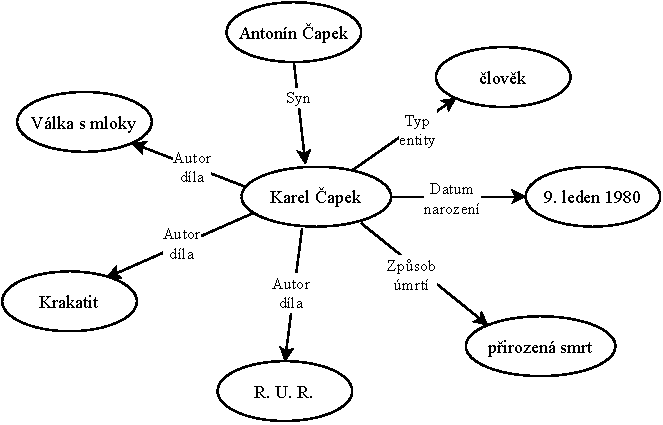
\includegraphics{media/capek-full.pdf}
    \caption{Ukázka části grafu jež může reprezentovat Karla Čapka.}
    \label{fig:capek-full}
\end{figure}

Jak vidíme z obrázku \ref{fig:capek-full}, zobrazit všechna data k vrcholu může být velmi nepřehledné a takovýchto vrcholů může být stovky. Pokud nás například zajímají pouze díla Karla Čapka, určitě v grafu nebudeme chtít mít informaci, že je Karel Čapek člověk. Tuto situaci můžeme vyřešit tak, že se na entity grafu budeme dívat pouze určitým pohledem a tedy zobrazíme pouze ty vztahy k vrcholu, jež odpovídají danému pohledu.

Kupříkladu pokud bychom chtěli procházet rodokmenem, je vhodné se na Karla Čapka dívat jako na osobu, jež má rodiče a sama může být rodičem ostatních osob. V tuto chvíli nás nezajímají ostatní vlastnosti jako knihy, které napsal, nebo ocenění, která získal. Na Karla Čapka se ale můžeme dívat i jako na spisovatele, kde nás pak zajímají pouze jeho díla a rodinné vztahy můžeme skrýt. Příklad takovýchto pohledů je na obrázku \ref{fig:capek-part}.

\begin{figure}[h]
    \centering
    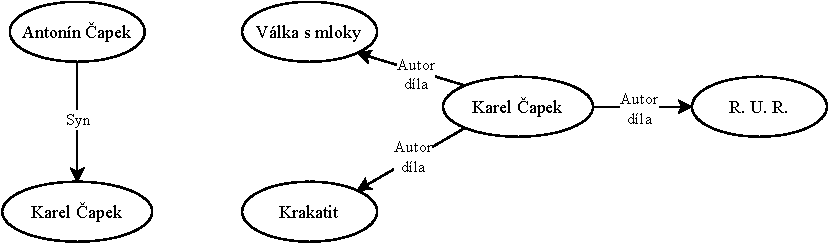
\includegraphics{media/capek-part.pdf}
    \caption{Pohled na Karla Čapka jako na osobu mající rodinu (vlevo) a na spisovatele jež je autorem literárních děl (vpravo)}
    \label{fig:capek-part}
\end{figure}

Tento způsob procházení grafových dat sice vyžaduje předem nadefinovat pohledy, ale procházení dat je pak jednoduché a velmi přehledné.

\section{Cíl práce}

Cílem této práce je vyrobit webovou aplikaci, jež by na základě předem definovaných pohledů vizualizovala grafová data a umožňovala uživateli procházet tento graf a objevovat nové vrcholy. Protože je žádoucí mít více pohledů na konkrétní typ vrcholu, pohledy jsou seskupeny do takzvaných konfigurací. Konfigurace pak popisuje nejen pohledy na různé typy vrcholů, ale i jaké vrcholy lze takto vizualizovat a z jakých zdrojů čerpat.

Konfigurace, jež jsou použité v aplikaci jsou například:
\begin{itemize}
    \item \textbf{Procházení živočichů na Wikidatech} - Uživatel může vizualizovat jednotlivé rostlinné a živočišné druhy a procházet je podle rozdělení do taxonů.
    \item \textbf{Procházení slavných osobností na Wikidatech} - Uživatel může procházet slavné osobnosti a nechat si načíst jejich filmová a literární díla a rodinné vztahy.
\end{itemize}

Motivací pro tuto práci je i výzkum\footnote{\citet{Klimek2019}} z roku 2019, jež dochází k závěru, že vizualizační nástroje, které by vyžadovaly malou znalost uživatele týkající se technických detailů RDF, chybí. Tato práce si klade za cíl odstínit běžného uživatele od těchto technických detailů, avšak bude obsahovat možnosti i pro technicky zdatnější uživatele, jež RDF rozumí.

\chapter{Technické předpoklady}

\section{Resource Description Framework}
Resource Description Framework, zkráceně RDF, je rodina specifikací\footnote{\citet{Raimond:14:RP}} (tedy sada pravidel), která se používá na popis informací na internetu. RDF popisuje data jako graf, konkrétně vrcholy grafu jsou entity, jež ztvárňují nějaké věci (fyzické předměty, díla, myšlenky) a hrany tyto entity propojují a dávají jim vztahy.

Základem je takzvaný \textbf{statement} (česky tvrzení). Tvrzení je vyjádřeno formou trojice v tomto pořadí ze subjektu, predikátu a objektu, přičemž subjekt a objekt jsou vrcholy (anglicky \textbf{nodes}) a predikát je orientovanou hranou jdoucí od subjektu k objektu.

Vrcholem v RDF může být IRI, literál, nebo prázdný uzel.

\medskip

Jako vrchol IRI (Internationalized Resource Identifier) se rozumí vrchol jež přiřazuje entitě nějaký identifikátor ve tvaru IRI. Tímto jsme schopni v rámci WWW identifikovat různé entity a pracovat s nimi napříč různými zdroji. Ku příkladu Karel Čapek, zmíněný v úvodu, je v rámci Wikidat jednoznačně identifikován jako \url{https://www.wikidata.org/wiki/Q155855}. IRI kromě identifikátoru nenese žádné další informace včetně jména, reprezentuje tedy nějakou entitu, která musí být popsaná tvrzeními, aby dostala význam.

\medskip

Literálem je pak uzel nesoucí nějakou hodnotu. Může se jednat o číslo popisující věk osoby, její jméno atp. V rámci RDF kromě hodnoty má literál i svůj typ, jež je opět vyjádřen pomocí IRI. Uveďme kupříkladu \url{http://www.w3.org/2001/XMLSchema#integer} jež vyjadřuje obecně celé číslo. Speciálním typem je \url{http://www.w3.org/1999/02/22-rdf-syntax-ns#langString} který vyžaduje ještě takzvaný \textbf{laguage tag} a popisuje text v nějakém konkrétním jazyce.

\medskip

Literály nám tedy dávají možnost přidat IRI uzlům různé hodnoty a podporují právě i multijazyčnost. Takovéto grafy pak dokáží popsat celou řadu věcí z reálného světa.

Nakonec, hrana je opět popsána pomocí IRI, jež reprezentuje typ vztahu.

\subsection{Turtle jazyk}
RDF graf může být popsán pomocí Turtle jazyka\footnote{\citet{Prud'hommeaux:14:RT}}. Ten je využit při zápisu konfigurací, jež jsou popsány dále v tomto dokumentu.

Trojice (tvrzení) se zapisují jako tři slova oddělená mezerami a zakončená tečkou. Chceme-li zapsat IRI, musíme jej dát do špičatých závorek \texttt{<>}. Na začátku dokumentu lze definovat prefixy, které pak umožňují zkrátit zapisované IRI do namespace a zbylé části \texttt{namespace:zbytek}.

Pokud se nám u trojic opakuje subjekt a predikát, můžeme jednotlivé objekty oddělovat čárkou (\texttt{,}). Obdobně, pokud se nám opakuje jen subjekt, můžeme dvojice predikát-objekt oddělovat středníkem (\texttt{;}).

\newpage

Uveďme několik příkladů RDF grafu.

\begin{prikl}
Tvrzení \uv{Karel Čapek se narodil 9. ledna 1890} vyjádřené v rámci Wikidat.
\begin{code}
@prefix wd: <https://www.wikidata.org/wiki/> .
@prefix wdt: <https://www.wikidata.org/wiki/Property:> .
@prefix xsd: <http://www.w3.org/2001/XMLSchema#> .

wd:Q155855 wdt:P569 "1890-01-09"^^xsd:dateTime .
\end{code}

Kód popisuje jedno tvrzení, kdy se Karlu Čapkovi \\ \url{https://www.wikidata.org/wiki/Q155855} přiřadí přes property datum narození \url{https://www.wikidata.org/wiki/Property:P569} literál s jeho datem narození, jež má typ \url{http://www.w3.org/2001/XMLSchema#dateTime}.
\end{prikl}

Jak lze vidět z příkladu, tvrzení nemusí odkazovat jen na svůj dataset, ale i mimo něj. To nám dovoluje stavět již na existujících datasetech a jednoduše se na ně okazovat přes IRI. Můžeme tak mít vlastní knihovní databázi jež ke knize přiradí autora z datasetu Wikidat. Tímto jsme propojili dva datasety, což nám umožní nad nimi provádět dotazy. Příkladem takového dotazu by mohlo být \uv{Chci seznam knih v naší knihovně, jež byly napsány českými autory.} Takový dotaz pak současně prohledá dva různé datasety a vrátí očekávané výsledky.

Uveďme ještě příklad tvrzení, jež se odkazuje na další entity.
\begin{prikl}
Tvrzení \uv{Děti Antonína Čapka jsou Karel, Josef a Helena} vyjádřené v rámci Wikidat.
\begin{code}
@prefix wd: <https://www.wikidata.org/wiki/> .
@prefix wdt: <https://www.wikidata.org/wiki/Property:> .

wd:Q6657059 wdt:P40 wd:Q155855 ,
                    wd:Q454568 ,
                    wd:Q4532606 .
\end{code}
\end{prikl}

\begin{figure}[h]
    \centering
    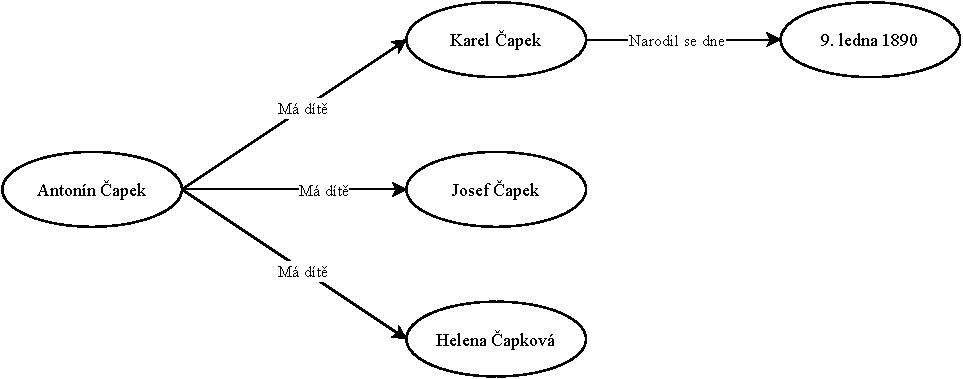
\includegraphics[width=\textwidth]{media/rdf.pdf}
    \caption{Příklad grafu který získáme z předešlých dvou ukázek.}
\end{figure}

Pro úplnost zmiňme ještě následující graf popisující vztahy mezi lidmi, které jsou vyjádřeny ontologií FOAF (friend of a friend). Pokud by všechny zdroje popisující lidi využívaly tuto ontologii, měli bychom jednotné rozhraní, jak přistupovat k lidským vztahům.

Ontologie je slovník obsahující formalizovaný seznam pojmů na definici kategorií a vztahů z určitého oboru.

\begin{code}
@prefix foaf: <http://xmlns.com/foaf/0.1/> .
@prefix example: <http://example.org/> .

<http://example.org/Jan-Novák> foaf:name "Jan Novák" .
<http://example.org/Ondřej-Novák> foaf:name "Ondřej Novák" .

example:Pavel-Novotný foaf:name "Pavel Novotný" ;
                      foaf:knows example:Jan-Novák ,
                                 example:Ondřej-Novák .
\end{code}

\subsection{SPARQL jazyk}
Jazyk SPARQL\footnote{\citet{Seaborne:13:SQL}} slouží k definici dotazů nad RDF daty a jejich manipulaci.

SPARQL má 4 typy dotazů:
\begin{itemize}
    \item \texttt{SELECT} dotaz vrací data z databáze ve formě tabulky obdobně jako u tabulkových databází. Můžeme tak například k jedné entitě vrátit hned několik vlastností jako různé sloupce tabulky.
    \item \texttt{CONSTRUCT} dotaz vrací data ve formě RDF grafu. Tento dotaz tedy použijeme, pokud chceme s výsledkem dále pracovat jako s grafem.
    \item \texttt{ASK} dotaz vrací pravdivostní hodnotu ano/ne podle toho, zda dotaz uspěl. Může být využit například ke zjištění, zda se konkrétní data již v databázi nacházejí.
    \item \texttt{DESCRIBE} dotaz obdobně jako \texttt{CONSTRUCT} vrací RDF graf s tím rozdílem, že zde určuje databáze, jaká data na dotaz dostaneme. Tento dotaz použijeme, pokud neznáme strukturu grafu a chceme získat \uv{nějaké} informace o vrcholu.
\end{itemize}

\newpage

\begin{prikl}
Dotaz, jež nám vrátí seznam děl Karla Čapka a jejich data vydání z Wikidat.
\begin{code}
PREFIX wd: <https://www.wikidata.org/wiki/>
PREFIX wdt: <https://www.wikidata.org/wiki/Property:>

SELECT ?title ?publication_date
WHERE
{
    wd:Q155855 wdt:P800 ?work .
    ?work wdt:P1476 ?title ;
          wdt:P577 ?publication_date .
}
\end{code}
Jedná se o \texttt{SELECT} dotaz, tedy jako výsledek dostaneme tabulku, jež má sloupce \texttt{title} a \texttt{publication_date}.

Dotaz se nejprve zeptá na všechny vrcholy, které dostaneme přes vlastnost \texttt{wdt:P800}, kterou Wikidata definují jako \uv{dílo - významné vědecké, umělecké či jiné dílo}. Tyto vrcholy jsou pak reprezentovány proměnnou \texttt{?work}. Na dalších dvou řádcích se pak dotazujeme, jaký titulek (\texttt{wdt:P1476}) má \texttt{?work} a uložíme ho do \texttt{?title}, který je i prvním sloupcem výstupu. Dále se pak obdobně ptáme na datum publikace, které je také součástí výsledku.
\end{prikl}
\chapter{Analýza požadavků}

\textit{Tato kapitola popisuje požadavky, jež byly kladeny na vývoj systému.}

Cílem práce je vyrobit webovou aplikaci, která vizualizuje grafová data dle předem definovaných konfigurací a je schopna s těmito daty pracovat. Konfigurace popisují jak a která data mají být vizualizována a jak je možné graf dále rozšiřovat. Celá aplikace bude rozdělena na klientskou a serverovou část, přičemž server odstiňuje klienta od RDF modelu a vrací mu již zpracovaná data.

Součástí požadavků na webovou aplikaci bylo vedoucím této práce připraveno několik konfigurací a webový server s určeným rozhraním, se kterým má klientská aplikace komunikovat.

V následujících kapitolách je nejprve popsána struktura konfigurací, rozhraní serveru a následně uživatelské požadavky na klientskou část aplikace.

\section{Konfigurace}

\textbf{Konfigurace} popisuje určitý pohled na data a definuje, jaká data lze v rámci této konfigurace vizualizovat a jakými způsoby. Konfigurace má \textbf{množiny pohledů}, kdy každá množina je aplikovatelná jen na určitou skupinu typů vrcholů podporovaných konfigurací. Množina pohledů pak obsahuje jednotlivé \textbf{pohledy}, které popisují, jak se na konkrétní vrchol můžeme dívat. Každý pohled pak určuje \textbf{náhled} (preview), \textbf{detail} a \textbf{expanzi}. Náhled poskytuje základní informace o vrcholu v rámci pohledu a určuje, jak má být vrchol v grafu vykreslen. Detail pak tyto informace rozšiřuje o další, které mohou být vypsány v tabulce. Expanze popisuje RDF graf, který doplňuje konkrétní vrchol o nové vztahy v rámci pohledu.

Konfigurace také určuje \textbf{počáteční vrchol} a \textbf{stylesheet}, tedy pravidla, jak mají být uzly v aplikaci vizualizovány.

Nakonec, konfigurace mohou být uloženy v rámci \textbf{meta konfigurací}, které slouží jako složky pro konfigurace.

Obrázek \ref{fig:configuration-class-diagram} popisuje UML diagram konfigurací.

\begin{figure}
    \centering
    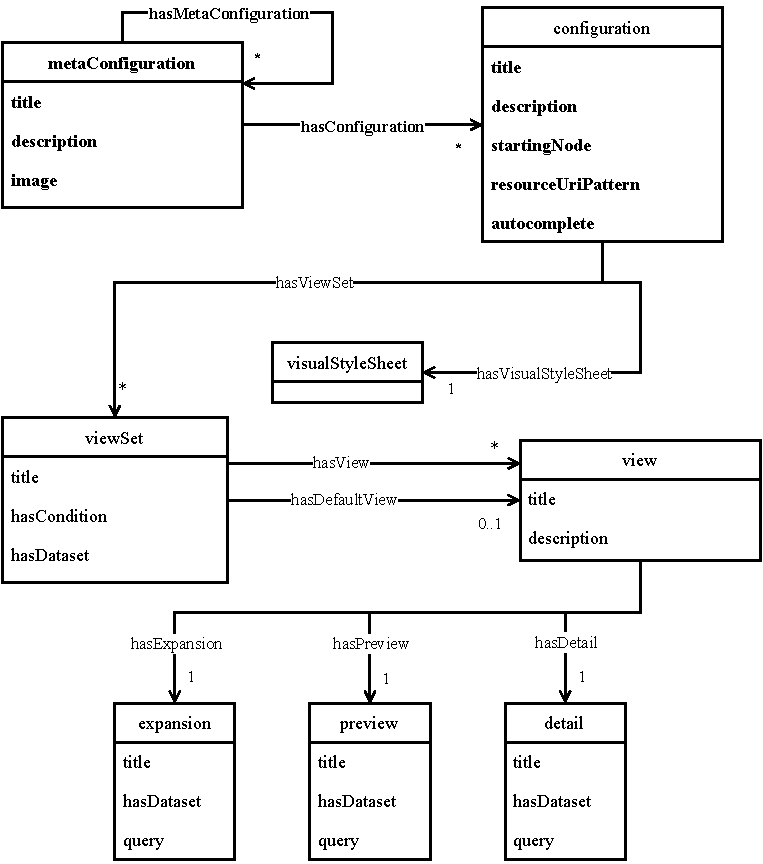
\includegraphics{media/configuration-class-diagram.pdf}
    \caption{Class diagram konfigurací včetně pozdější implementace meta konfigurace a rozšíření konfigurace.}
    \label{fig:configuration-class-diagram}
\end{figure}

\bigskip

V následujících sekcích jsou použity tyto RDF namespacy:
\begin{table}[h] \centering
\begin{tabular}{lp{10cm}}
\toprule
\multicolumn{1}{c}{Prefix} & \multicolumn{1}{c}{IRI}                                      \\
\midrule
browser                    & \texttt{\url{https://linked.opendata.cz/ontology/knowledge-graph-browser/}} \\
dct                        & \texttt{\url{http://purl.org/dc/terms/}}
\end{tabular}
\end{table}

\newpage

\subsection{Meta konfigurace} \label{pozadavky-metakonfigurace}
Meta konfigurace je skupina pro další konfigurace a meta konfigurace. Díky tomuto může uživatel procházet desítky různých konfigurací uspořádaných do složek obdobně jako v souborovém systému na počítači. Meta konfigurace má tyto vlastnosti:

\begin{itemize}
    \item \texttt{dct:title} Název meta konfigurace. \textit{(je možné zadat ve více jazycích)}
    \item \texttt{dct:description} Detailnější popis, co daná meta konfigurace zahrnuje. \textit{(je možné zadat ve více jazycích)}
    \item \texttt{browser:image} URL adresa s obrázkem reprezentující meta konfiguraci. Obrázek je pak zobrazen v aplikaci při procházení konfigurací.
    \item \texttt{browser:hasMetaConficuration} Meta konfigurace, které spadají pod tuto meta konfiguraci. \textit{(je očekáváno více objektů)}
    \item \texttt{browser:hasConfiguration} Konfigurace, které spadají pod tuto meta konfiguraci. \textit{(je očekáváno více objektů; popsáno dále)}
\end{itemize}

Meta konfigurací může být například \uv{Wikidata} nebo \uv{Otevřená data ČR}.

\subsection{Konfigurace} \label{pozadavky-konfigurace}
Konfigurace popisuje způsoby, jakými se lze dívat na data. Dvě konfigurace již byly zmíněny v úvodní kapitole. Aktuálně může mít konfigurace tyto vlastnosti:

\begin{itemize}
    \item \texttt{dct:title} Název konfigurace. \textit{(je možné zadat ve více jazycích)}
    \item \texttt{dct:description} Detailnější popis čeho je možné s konfigurací dosáhnout. \textit{(je možné zadat ve více jazycích)}
    \item \texttt{browser:hasVisualStyleSheet} Určuje, jak mají být uzly v aplikaci vizualizovány. \textit{(popsáno dále)}
    \item \texttt{browser:startingNode} Doporučený uzel nebo uzly, se kterými začít s procházením grafu. \textit{(je očekáváno více objektů)}
    \item \texttt{browser:resourceUriPattern} Regulární výraz popisující, jak by mělo vypadat IRI uzlu. Používá se v aplikaci jako nápověda uživateli, zda zadal správné IRI dřív, než se pošle požadavek. Také se používá pro sestavení IRI z vyhledávaného dotazu, pokud lze dotazem nahradit část výrazu a získat tak validní IRI.
    \item \texttt{browser:hasViewSet} Seznam množin pohledů které tato konfigurace podporuje. \textit{(popsáno dále)}
    \item \texttt{browser:autocomplete} JSON soubor se seznamem RDF uzlů podle kterých probíhá hledání. \textit{(je očekáváno více objektů; popsáno dále)}
\end{itemize}

\subsection{ViewSet} \label{pozadavky-view-sets}
View set reprezentuje skupinu pohledů. Skupina pohledů je vždy aplikovatelná na určité typy vrcholů v rámci konfigurace. View set má následující vlastnosti:
\begin{itemize}
    \item \texttt{dct:title} Název view setu. \textit{(je možné zadat ve více jazycích)}
    \item \texttt{browser:hasView} Pohledy, které patří pod tento view set. \textit{(je očekáváno více objektů; popsáno dále)}
    \item \texttt{browser:hasDefaultView} Výchozí pohled ze seznamu výše.
    \item \texttt{browser:hasCondition} SPARQL ASK dotaz jež určí, zda tato množina pohledů je aplikovatelná na konkrétní vrchol.
    \item \texttt{browser:hasDataset} Dataset, vůči kterému probíhá ASK dotaz. \textit{(popsáno dále)}
\end{itemize}

\subsection{View} \label{pozadavky-view}
Konkrétní pohled na vrchol, který určuje náhled, detail a expanzi. Jak již bylo zmíněno v úvodu, pohledem může být například \uv{člověk, jež je autorem literárních děl}, nebo \uv{člověk jako součást rodokmenu}. View má následující vlastnosti:

\begin{itemize}
    \item \texttt{dct:title} Název pohledu. \textit{(je možné zadat ve více jazycích)}
    \item \texttt{dct:description} Popis pohledu. \textit{(je možné zadat ve více jazycích)}
    \item \texttt{browser:hasExpansion} Expanze -  popisuje graf který rozšiřuje vrchol o nové vrcholy v rámci daného pohledu. \textit{(popsáno dále)}
    \item \texttt{browser:hasPreview} Preview (náhled) - určuje data která popisují vrchol v rámci daného pohledu a na základě kterých se vrchol vizuálně vykreslí \textit{(popsáno dále)}
    \item \texttt{browser:hasDetail} Detail - určuje dodatečné informace o vrcholu v rámci daného pohledu. \textit{(popsáno dále)}
\end{itemize}

\subsection{Expanze} \label{pozadavky-expansion}
Expanze popisuje, jak lze daný vrchol rozšířit o nové vrcholy, které s ním souvisí. Expanze vrací graf, tedy expandované uzly nemusí být přímými sousedy expandovaného vrcholu. Jako expanzi si můžeme představit například \uv{Zobraz všechny knihy, co napsala daná osoba}. Expanze formálně partří k pohledu (view).
\begin{itemize}
    \item \texttt{dct:title} Název expanze. \textit{(je možné zadat ve více jazycích, aktuálně se nepoužívá)}
    \item \texttt{browser:hasDataset} Popisuje dataset, vůči kterému se dotazuje na data. \textit{(popsáno dále)}
    \item \texttt{browser:query} Popisuje SPARQL CONSTRUCT dotaz, který bude spuštěn na endpointu datasetu a vrátí výsledný graf.
\end{itemize}

\subsection{Preview (náhled)} \label{pozadavky-preview}
Preview určuje, která data v rámci daného pohledu (view) popisují konkrétní vrchol. Popisem se myslí taková data, podle kterých se určí, jak bude vrchol na grafu vizuálně vykreslen. Obdobně jako expanze, preview patří ke konkrétnímu pohledu.

Preview má stejné vlastnosti jako expanze. \texttt{browser:query} v tomto případě popisuje SPARQL CONSTRUCT dotaz, který vrátí graf obsahující daný uzel společně s literály ze kterých bude sestaven preview.

Konkrétně pro preview je predikát \texttt{browser:class} považován za třídu uzlu. Podle těchto tříd je pak možné nastavovat vizuální styly pro konkrétní vrcholy.

\subsection{Detail} \label{pozadavky-detail}
Detail poskytuje dodatečné informace k uzlu. Může se jednat o literály, které nemá smysl v dané konfiguraci vykreslit do grafu jako uzly, a proto budou zobrazeny v bočním panelu aplikace po kliknutí na uzel.

Detail má stejné vlastnosti včetně \texttt{browser:query} jako preview.

\subsection{Dataset} \label{pozadavky-dataset}
Dataset popisuje SPARQL endpoint vůči kterému probíhá dotazování na data.

\begin{itemize}
    \item \texttt{dct:title} Název datasetu. \textit{(aktuálně se nepoužívá)}
    \item \texttt{void:sparqlEndpoint} URL adresa SPARQL endpointu na kterou se posílají dotazy.
    \item \texttt{browser:accept} Popisuje HTTP Accept type - v jakém formátu by měl endpoint svá data poskytnout.
\end{itemize}

\subsection{Visual style sheet} \label{pozadavky-visual-style-sheet}
Popisuje sadu pravidel, podle kterých budou vizuálně vykresleny vrcholy v aplikaci. Pravidla popsaná v rámci style sheetu mohou pracovat náhledem (preview) včetně zmíněných tříd. Forma zápisu stylů aktuálně odpovídá stylům, jaké používá knihovna Cytoscape\footnote{\url{https://js.cytoscape.org/}}, která bude popsána v další kapitole.

Visual style sheet má pouze jednu vlastnost

\begin{itemize}
    \item \texttt{browser:hasVisualStyle} Pravidlo popisující, jak se má provést stylování. Odkazuje na \textbf{Visual style}.
\end{itemize}

\subsubsection{Visual style}
Visual style má pak:

\begin{itemize}
    \item \texttt{browser:hasSelector} Selector pro Cytoscape knihovnu, jež vybírá, \\ na které uzly nebo hrany bude daný styl aplikován.
    \item \texttt{browser:*} Konkrétní styly, jak má být daný uzel vykreslen. Používají se přesně ty názvy, které používá knihovna Cytoscape. Kupříkladu \\\texttt{browser:border-width} nebo \texttt{browser:background-color}.
\end{itemize}

\bigskip

Vedoucím projektu byly dodány pouze konfigurace. Výše sepsaná dokumentace konfigurací je již součástí této práce.

Původní návrh konfigurací byl mírně jednodušší a považoval konfigurace pouze jako odkazy na seznam pohledů. Klientská aplikace tedy musela mít seznam konfigurací s jejich názvy, počátečními vrcholy a dalšími parametry.

Na základě debaty s vedoucím byla konfigurace rozšířena o meta konfigurace a o parametry u konfigurace, jako název, popisek, počáteční vrcholy atp. To nám umožnilo mít v rámci klientské aplikace pouze jeden odkaz na IRI meta konfigurace, ze které se dají získat další meta konfigurace a konfigurace. Je tedy možné přidávat konfigurace bez nutnosti měnit klientskou část aplikace.

\bigskip

\begin{prikl}
Na závěr uveďme část konfigurace popisující procházení taxonů živočichů a rostlin na Wikidatech. Tato konfigurace je dostupná pod IRI \\\href{https://linked.opendata.cz/resource/knowledge-graph-browser/configuration/wikidata/animals}{https://linked.opendata.cz/resource/knowledge-graph-browser/}\\\href{https://linked.opendata.cz/resource/knowledge-graph-browser/configuration/wikidata/animals}{configuration/wikidata/animals}. Prefix \texttt{rb} definujme jako \\\url{https://linked.opendata.cz/resource/knowledge-graph-browser/}.

\smallskip

\textbf{Definice konfigurace}
\begin{code}
rb:configuration/wikidata/animals
    a browser:Configuration ;
    dct:title "Taxonomy of animals and plants"@en ,
              "Taxonomie rostlin a živočichů"@cs ;
    browser:hasVisualStyleSheet
        rb:wikidata/animals/style-sheet ;
    browser:startingNode <http://www.wikidata.org/entity/Q7377> ,
                         <http://www.wikidata.org/entity/Q192154> ;
    browser:resourceIriPattern
        "^http://www\\.wikidata\\.org/entity/Q[1-9][0-9]*$" ;
    browser:hasViewSet
        rb:view-set/wikidata/animals/taxon .
\end{code}

\textbf{Definice pohledu}
\begin{code}
rb:view/wikidata/animals/taxon/narrower a browser:View ;
    dct:title "Child taxons"@en ;
    browser:hasExpansion rb:expansion-query/animals/taxon/narrower ;
    browser:hasPreview rb:preview-query/animals/taxon/basic ;
    browser:hasDetail rb:detail-query/animals/taxon/basic .
\end{code}

\textbf{Definice datasetu}
\begin{code}
rb:dataset/wikidata a void:Dataset ;
    dct:title "Wikidata SPARQL endpoint" ;
    void:sparqlEndpoint <https://query.wikidata.org/sparql> ;
    browser:accept "application/sparql-results+json" .
\end{code}

\textbf{Definice stylu}
\begin{code}
rb:wikidata/animals/style/genus a browser:VisualStyle ;
    browser:background-color "#ffbf00" ;
    browser:hasSelector ".genus" .
\end{code}
\end{prikl}


\section{Server}
Dalším požadavkem bylo, aby klientská aplikace komunikovala se serverem, který provádí dotazy a vrací data pro aplikaci. Server bude detailněji popsán v příští kapitole.

Server zprostředkovává následující požadavky:
\begin{itemize}
    \item \texttt{/meta-configuration} - Vrátí informace o meta konfiguraci.

    \item \texttt{/configuration} - Vrátí informace o konfiguraci.

    \item \texttt{/stylesheet} - Vrátí visual style sheet.

    \item \texttt{/view-sets} - K vrcholu a konfiguraci vrátí seznam view setů.

    \item \texttt{/preview} - K vrcholu a pohledu vrátí preview.

    \item \texttt{/detail} - K vrcholu a pohledu vrátí detail.

    \item \texttt{/expand} - K vrcholu a pohledu vrátí expandované uzly.
\end{itemize}

\newpage







\begin{figure}
    \centering
    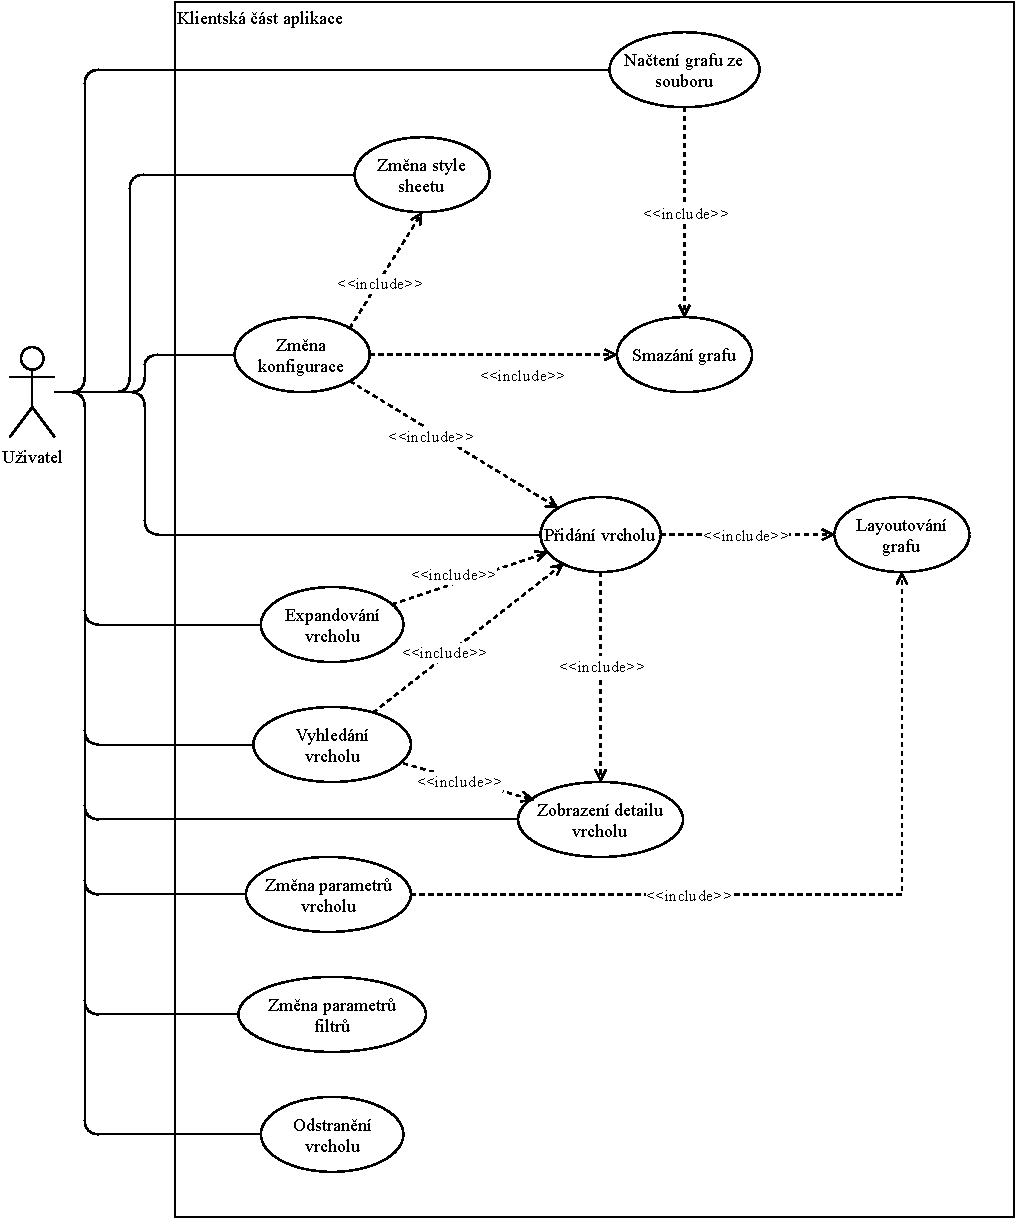
\includegraphics[width=\textwidth]{media/use-case.pdf}
    \caption{Use case diagram dle uživetelských požadavků.}
    \label{fig:use-case}
\end{figure}

\section{Uživatelské a systémové požadavky}

Níže je sepsán seznam původních požadavků na klientskou aplikaci.

\subsection*{Konfigurace a stylesheet}
Uživatel musí být schopen vybrat IRI konfigurace a IRI visual style sheetu a lze je kdykoli změnit. IRI konfigurace může být vybráno jen jedno.

\paragraph{Analýza} Konfigurace popisuje, jak je graf zobrazen a které pohledy jsou na uzly aplikovatelné. Ačkoli by teoreticky bylo možné podporovat dvě konfigurace, nebudeme toto implementovat. Změna konfigurace tedy smaže aktuální graf a vytvoří graf nový.

\subsection*{Vložení vrcholů}
Uživatel může ručně zadat IRI vrcholu, který se následně zobrazí v grafu.

\paragraph{Analýza} Pro úspěšné zobrazení vrcholu musí aplikace znát jeho \texttt{preview}. To lze ale získat pouze z konkrétního pohledu a je tedy nutné nejprve stáhnout \texttt{view-sets} daného vrcholu, z nich následně vybrat defaultní a zvolit výchozí pohled. Pak je možné zavolat metodu \texttt{preview} na serveru a získat data o vrcholu.

\begin{itemize}
    \item IRI vrcholu bude považováno za chybné, pokud server vrátí prázdnou množinu na dotaz \texttt{view-sets}. V takovém případě totiž nejde aplikovat žádné pohledy na uzel, a tedy zřejmě nepatří do dané konfigurace.
    \item Vrchol může být již v grafu přítomen, pak se označí a přesune se na něj obrazovka. Pokud je vrchol skrytý, bude odkryt. Pokud jsou zapnuté filtry a vrchol je skrytý filtrem, vrchol se v grafu nezobrazí. Pokud se vrchol podaří načíst, nebo již existuje, bude vybrán a zobrazí se jeho detail v pravém panelu.
\end{itemize}

\subsection*{Detail vrcholu}
Pokud uživatel klikne na vrchol, zobrazí se panel s podrobnými informacemi o uzlu. Bude zobrazen detail uzlu voláním metody \texttt{detail} na serveru a budou zobrazeny veškeré pohledy vrcholu, možnost je přepínat a provádět expanze podle daného pohledu.

Detail bude zobrazen jako dvousloupcová tabulka klíč-hodnota.

Panel bude zobrazovat také další možné akce k vrcholu.

\paragraph{Analýza} Vrchol nemusí mít načtené \texttt{view-sets}, \texttt{preview} ani \texttt{detail}, je tedy nutné po zobrazení panelu tyto informace stáhnout a během stahování zobrazit informaci, že se data stahují.

Může se stát, že \texttt{view-sets} vrátí prázdný výsledek. V takovém případě vrchol v grafu necháme i přes to, že podle původního požadavku bychom jej smazali. Taková situace nicméně implikuje chybně napsanou konfiguraci a uživatel bude o tomto informován chybovou hláškou.

Mezi akcemi bude lokalizace vrcholu, smazání, znovunačtení všech dat, zafixování pozice.

\subsection*{Skrývání uzlů}
Uživatel může skrývat uzly v panelu s detailem. Skrytý uzel se v grafu skryje společně se všemi hranami. Bude možné zobrazit seznam skrytých uzlů ze kterého půjde skryté uzly opět zviditelnit.

\paragraph{Analýza} Bude přidáno tlačítko k detailu pro skrytí/zobrazení uzlu. Současně pro vetší přehlednost bude do detailu přidána hláška informující uživatele, že je uzel skrytý.

Skryté uzly nebude možno lokalizovat, ale stále bude možné s nimi dále pracovat. Podle prvního požadavku se uzel opět zobrazí, pokud ho uživatel bude chtít explicitně vložit.

V panelu se skrytými uzly bude možnost uzly přímo zobrazit, nebo si zobrazit jejich detail. Detail skrytého uzlu funguje stejně jako pro viditelné uzly.

\subsection*{Expanze}
Po dvojkliku na uzel se uzel expanduje podle aktuálního pohledu. Uzel je také možné expandovat v panelu s detailem kliknutím na tlačítko expanze u příslušného pohledu. Expanzí se zavolá metoda \texttt{expand} na serveru a v grafu se zobrazí nové vrcholy.

\paragraph{Analýza} Pokud přidávaný vrchol v grafu již je a je skrytý, pak skrytým zůstane. Na rozdíl od přidávání jednoho vrcholu totiž explicitně neříkáme, že chceme daný vrchol přidat. Protože je možné vrcholy mazat, povolíme uživateli provádět expanzi znova, i když již byla provedena.

Budeme si také pamatovat které vrcholy a hrany vznikly ze které expanze pro snazší práci s expanzemi.

\subsection*{Filtrování vrcholů}
Uživatel může přidat filtr, jež skryje nevyhovující vrcholy. Takovéto skryté vrcholy se pak chovají stejně jako uživatelem skryté vrcholy. Požadované filtry jsou
\begin{itemize}
    \item Zobraz jen ty vrcholy, jež mají stupeň v daném intervalu nebo rozmezí.
    \item Zobraz vrcholy jen s konkrétním typem nebo třídou.
\end{itemize}

\paragraph{Analýza} Aplikace by měla podporovat snadné přidání filtrů do budoucna a podporu pro pluginy, které dodávají vlastní možnosti filtrování. Aby bylo možné vyjádřit libovolné filtry, každý filtr by měl mít přístup k celému grafu a všem vrcholům.

Uzel může být skrytý jak filtrem, tak i uživatelem. Pro přehlednost by měl být uživatel informován, že nemůže ručně zobrazit vrchol který je skrytý filtrem. Tyto vrcholy budou stále zobrazeny v seznamu skrytých vrcholů pro možnost přístupu k nim.

Každý filtr určí, zda je vrchol podle tohoto filtru viditelný. Vrchol pak bude viditelný, pokud všechny filtry určí, že viditelný je. Jedná se tedy o konjunkci.

Typy a třídy vrcholů nejsou známy předem a API serveru neumožňuje získat celou množinu typů a tříd. Je tedy nutné přizpůsobit filtry tak, aby si dokázaly poradit s novými uzly. Proto filtry na typ a třídu budou mít dva módy. V jednom módu explicitně skrývají zvolené vlastnosti a ve druhém explicitně zobrazují vrcholy s danými vlastnostmi. Toto chování pak ovlivní přidání nových, neznámých, vrcholů. V prvním případě nový vrchol bude zobrazen (pokud jeho typ, resp. třídy ještě nejsou známy) a ve druhém případě bude ihned skryt.

\subsection*{Vícejazyčné uživatelské rozhraní}
Uživatel může přepínat mezi více jazyky uživatelského rozhraní. Aktuálně bude podporována pouze angličtina a čeština.

\paragraph{Analýza} Kromě uživatelského rozhraní by měl být vícejazyčný i graf. Aktuální API serveru toto ještě neumožňuje a problém je předmětem poslední kapitoly. Multijazyčnost zatím podporují metody \texttt{meta-configuration} a \texttt{configuration} na serveru. Protože obecně můžou existovat překlady do spousty světových jazyků, je vhodné stahovat pouze požadovaný jazyk a při jeho změně stáhnout data s novým jazykem znovu.

Pro velké grafy může být překlad problémem, protože změna jazyku může vyvolat spoustu požadavků na datové zdroje. Pro překlad grafu by tedy bylo nejlepší stáhnout překlad až když si uživatel zobrazí detail, nebo explicitně neoznačí vrcholy na překlad. Taktéž je vhodné oddělit výběr jazyka pro obsluhu aplikace a výběr konfigurací od překladu jednotlivých vrcholů. Příkladem situace, kde je oddělení žádoucí, může být procházení měst v Japonsku anglicky mluvícím uživatelem. V této situaci bychom požadovali, aby názvy měst byly v originálním jazyce.

Překlady do konkrétního jazyka by měly být v jednom souboru, nebo adresáři a přidávání nových jazyků by mělo být snadné, nejlépe bez zásahu do kódu aplikace.

\subsection*{Stažení grafu do souboru}
Uživatel má možnost stáhnout aktuální graf do souboru a později ho ze souboru načíst zpět.

\paragraph{Analýza} Protože je aplikace ve vývoji, je třeba dbát na zpětnou kompatibilitu. Při každé nové verzi je tedy třeba ověřit, zdali soubor pochází ze staré verze a použít staré metody pro jeho zpracování a převedení do nového systému. Výsledný soubor může být zkomprimován pro menší velikost a nabízí se i možnost stáhnout jen základní informace tak, aby zbytek mohl být při načtení stažen ze serveru.

Pokud uživatel bude chtít zavřít aplikaci, bude dotázán, zda chce aktuální graf uložit do souboru. Uložený graf již nebude blokovat stránku o uzavření, dokud uživatel nesmaže, nebo nepřidá nové uzly. Stažení detailu, nebo změna pohledu nebude považována za změnu hodnou k uložení.

Pokud uživatel zvolí načtení nového souboru, starý graf bude zahozen a uživatel tedy bude požádán o uložení.

Kromě otevření souboru ze systému bude možnost soubor načíst i z webu.

\subsection*{Odstranění vrcholu}
Uživatel může z grafu vrchol odstranit.

\paragraph{Analýza} Odstraněním vrcholu se musí odstranit i všechny hrany patřící vrcholu. Vrchol by také měl být odstraněn ze všech expanzí tak, aby nedocházelo k únikům paměti.

Odstranit vrchol bude možné pomocí tlačítka v panelu s detailem, popřípadě skupinu vrcholů bude možné odstranit obdobným způsobem.

\subsection*{Vyhledávání vrcholů s pomocí autocomplete}
Pokud to konfigurace umožňuje, bude možné přidávat nové uzly do grafu s pomocí autocomplete.

\paragraph{Analýza} Data pro vyhledávání se budou stahovat až když uživatel bude chtít poprvé vyhledávat.

Návrh vyhledávače by měl podporovat více vyhledávacích zdrojů a vhodně kombinovat nalezené výsledky v případě, že více zdrojů vrátí stejné vrcholy.

Kromě vyhledávání v JSON souboru se pak nabízí hledat i v aktuálním grafu a umožnit uživateli zadat do vyhledávacího pole přímo IRI uzlu, popřípadě její část, ze které se aplikace pokusí sestavit celou IRI.

\subsection*{Podpora layoutů}
Aplikace bude umožňovat několik způsobů layoutování grafu, které si bude moci uživatel volit.

\begin{itemize}
    \item Pokud to layout umožňuje, bude možné ukotvit vrchol. To lze provést přesunutím vrcholu, pravým kliknutím myši, nebo z nabídky u detailu vrcholu. U ukotvených vrcholů bude zobrazena ikonka. Takovéto vrcholy pak nebudou layoutem ovlivněny.
    \item Layout reaguje na různé události, jako vytvoření skupiny, expanze vrcholu, přidání nového vrcholu do grafu, přesunutí vrcholu a na základě těchto událostí provádí layoutování grafu.
    \item Pokud to layout umožňuje, bude v pravém dolním rohu obrazovky tlačítko, které spustí layoutování explicitně.
    \item Layout má vlastní nastavení.
\end{itemize}

\subsection*{Seskupování vrcholů}
Vrcholy bude možné seskupovat do skupin, které budou ve vizuálním grafu reprezentovány jedním vrcholem. Pokud expanze vrátí větší množství nových vrcholů, vzniknou jako skupina. Skupinu bude možné rozbít dvojklikem.

\begin{itemize}
    \item Z grafového hlediska skupina vznikne kontrakcí hran mezi vrcholy skupiny. To znamená, že pokud vedla hrana mezi vrcholem mimo skupinu a vrcholem ve skupině, povede tato hrana mezi vrcholem mimo skupinu a skupinou. Všechny násobné hrany stejného typu budou nahrazeny jednou hranou. Obdobně toto platí pro hrany mezi dvěma skupinami. Pokud je ve skupině vrchol skrytý (uživatelem, nebo filtrem), jeho hrany se nepodílejí na utváření skupiny. Pokud jsou všechny vrcholy skupiny skryty, je skrytá i skupina.
    \item Skupina se na grafu chová jako obyčejné vrcholy, je ji možné skrýt, přesouvat, ukotvit atp.
    \item Označením několika vrcholů se nabídne možnost vytvořit skupinu. Tato skupina pak vznikne na místě, kde byly původní vrcholy.
    \item Rozbít skupinu je možné dvojklikem, nebo tlačítkem z detailu skupiny. Vrchol skupiny bude odstraněn a vzniknou místo něj původní vrcholy, které budou layoutovány.
\end{itemize}

\subsection*{Kompaktní mód}
Uživatel bude mít možnost zapnout kompaktní mód. Během něj se ve středu obrazovky zobrazí pouze zvolené vrcholy a jejich přímí sousedi. Tyto vrcholy budou layoutovány bez ohledu na ostatní vrcholy, které budou skryté. Uživatel pak bude mít možnost graf v tomto módu procházet klikáním na sousedy aktivního vrcholu.

\paragraph{Analýza} Kompaktní mód se vypne, pokud nebude vybrán žádný vrchol. Při kompaktním módu se bude obrazovka neustále zaměřovat na vrcholy účastnící se kompaktního módu. Jamile vrchol kompaktní mód opustí, měl by se vrátit na svou původní pozici. Pak po skončení kompaktního módu se původní rozložení grafu nezmění. Nově vytvořené vrcholy v rámci kompaktního módu musí být i správně umístěny, jakmile bude mód ukončen.

\chapter{Návrh architektury}

Aplikace je rozdělena na serverovou a klientskou část. Server slouží pro odstínění klienta od RDF databází, komunikuje tedy přímo s datovými zdroji a zpracované data předává klientské aplikaci. Klient pak v případě potřeby z internetu stahuje externí obrázky (příkladem jsou konfigurace Wikidat, které obsahují URL odkazy) a autocomplete soubory.

Rozdělení aplikace na klient-server také umožňuje cachování na straně serveru, které ještě implementováno není. Tento problém je diskutován v poslední kapitole.

Server tak slouží na odstínění od link datové vrstvy a v budoucnu pro cachování dat, aktuálně je bezestavový.

\begin{figure}[h]
    \centering
    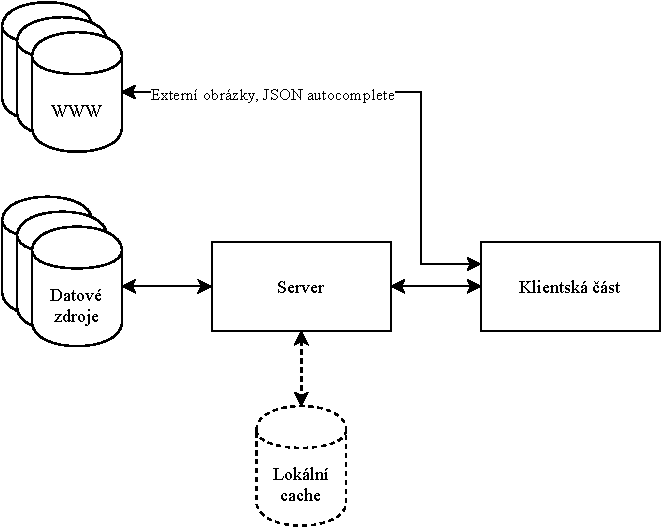
\includegraphics[width=0.75\textwidth]{media/communication.pdf}
    \caption{Komunikace mezi klientem, serverem a datovými zdroji. Cachování na serveru ještě implemontováno není.}
\end{figure}

\section{Server}
Jak již bylo v dokumentu zmíněno, převážná část serveru byla dodána jako specifikace pro klientskou aplikaci.

\subsection{Jazyková podpora} \label{jazykova-podpora}
Server jsem částečně přepsal, aby podporoval dotazování na data z více světových jazyků. Některé požadavky přijímají parametr \texttt{languages} obsahující čárkou (\texttt{,}) oddělené ISO 639-1 jazykové kódy. Server pak vrací objekty jejiž klíčem je jazykový kód a hodnotou daný překlad do jazyka. Pokud překlad neexistuje, hodnotou je \texttt{null}. V případě, že na všechny jazyky bylo vráceno \texttt{null}, server se pokusí přidat další jazyk, který existuje. Který jazyk takto bude vybrán není určeno.

Tato implementace umoňuje stahování vícejazyčných dat tak, že jsou stažené jen žádané jazyky, což může značně ušetřit přenos dat v některých případech, ale současně dojde ke stažení alespoň jednoho podporovaného jazyka, pokud je to možné.

\begin{prikl}
Pro \texttt{languages=cs,en} může server vrátit například
\begin{code}[frame=none]
{
    cs: null,
    en: "Kankakee County"
}
\end{code}
ale pokud nezná překlad ani do češtiny, ani do angličity, může vrátit
\begin{code}[frame=none]
{
    cs: null,
    en: null,
    sk: "Jazero Beňatina"
}
\end{code}
\end{prikl}

\subsection{API}
Server vrací data ve formátu JSON, požadavky jsou posílány metodou GET a parametry jsou kódovány do URL adresy.

\subsubsection{/metaconfiguration}
\textbf{parametry:} \texttt{iri} a \texttt{languages} \\
Vrátí informace o metakonfiguraci zadané podle \texttt{iri}. \\
Vrátí všechna data (viz kapitola \ref{pozadavky-metakonfigurace}) o metakonfiguraci, veškerá data o dceřiných konfiguracích (viz kapitola \ref{pozadavky-konfigurace}) a základní data o dceřiných metakonfiguracích (vše kromě seznamu konfigurací a metakonfigurací).

\begin{code}
interface ResponseMetaConfiguration extends
ResponseMetaConfigurationBase {
    has_meta_configurations: ResponseMetaConfigurationBase[],
    has_configurations: ResponseConfiguration[],
}

interface ResponseMetaConfigurationBase {
    iri: string,
    title: {[language: string]: string},
    description: {[language: string]: string},
    image: string,
}
\end{code}

\subsubsection{/configuration}
\textbf{parametry:} \texttt{iri} a \texttt{languages} \\
Vrátí informace o konfiguraci zadané podle \texttt{iri}. \\
Vrátí stejná data jako \texttt{/metaconfiguration} o svých sceřiných konfiguracích. \\
Toto volání se používá pouze když uživatel ručně zvolí IRI konfigurace, v opačném případě si aplikace vystačí s voláním \texttt{/metaconfiguration}.

\begin{code}
interface ResponseConfiguration {
    iri: string,
    stylesheet: string[],
    title: {[language: string]: string},
    description: {[language: string]: string},
    autocomplete: string[],
    starting_node: string[],
    resource_pattern: string|null,
}
\end{code}

\subsubsection{/stylesheet}
\textbf{parametry:} \texttt{stylesheet} \\
Vrátí kompletní visual style sheet (viz kapitola \ref{pozadavky-visual-style-sheet}) na základě jeho IRI jako parametr \texttt{stylesheet}.

\begin{code}
interface ResponseStylesheet {
    styles: {
        selector: string;
        properties: {
            [property: string]: string;
        }
    }[];
}
\end{code}

\subsubsection{/view-sets}
\textbf{parametry:} \texttt{config} a \texttt{resource} \\
Vrátí seznam možných view setů (viz kapitola \ref{pozadavky-view-sets}) které odpovídají uzlu s IRI \texttt{resource} při dané konfiguraci \texttt{config}.

\begin{code}
interface ResponseViewSets {
    viewSets: {
        iri: string;
        label: string;
        defaultView: string;
        views: string[];
    }[];
    views: {
        iri: string;
        label: string;
    }[];
}
\end{code}

\subsubsection{/preview}
\textbf{parametry:} \texttt{view} a \texttt{resource} \\
Vrátí data z dotazu preview (viz kapitola \ref{pozadavky-preview}) na uzel s IRI \texttt{resource} při daném pohledu \texttt{view}.

\begin{code}
interface ResponsePreview {
    nodes: ResponseElementNode[];
    types: ResponseElementType[];
}
\end{code}

\subsubsection{/detail}
\textbf{parametry:} \texttt{view} a \texttt{resource} \\
Vrátí data z dotazu detail (viz kapitola \ref{pozadavky-detail}) na uzel s IRI \texttt{resource} při daném pohledu \texttt{view}.

\begin{code}
interface ResponseDetail {
    nodes: {
        iri: string;
        data: {
            [IRI: string]: string;
        };
    }[];
    types: ResponseElementType[];
}
\end{code}

\subsubsection{/expand}
\textbf{parametry:} \texttt{view} a \texttt{resource} \\
Vrátí expandované uzly (viz kapitola \ref{pozadavky-expansion}) pro uzel s IRI \texttt{resource} při daném pohledu \texttt{view}. Tyto expandované uzly již obsahují data o detailu a tedy není třeba žádného dalšího volání.

\begin{code}
interface ResponseExpand {
    nodes: ResponseElementNode[];
    edges: ResponseElementEdge[];
    types: ResponseElementType[];
}
\end{code}

\newpage

Mezi pomocná rozhraní pak patří
\begin{code}
interface ResponseElementType {
    iri: string;
    label: string;
    description: string;
}

interface ResponseElementEdge {
    source: string;
    target: string;
    type: string;
    classes: string[];
}

interface ResponseElementNode {
    iri: string;
    type: string;
    label: string;
    classes: string[];
}
\end{code}

\begin{figure}[p]
    \centering
    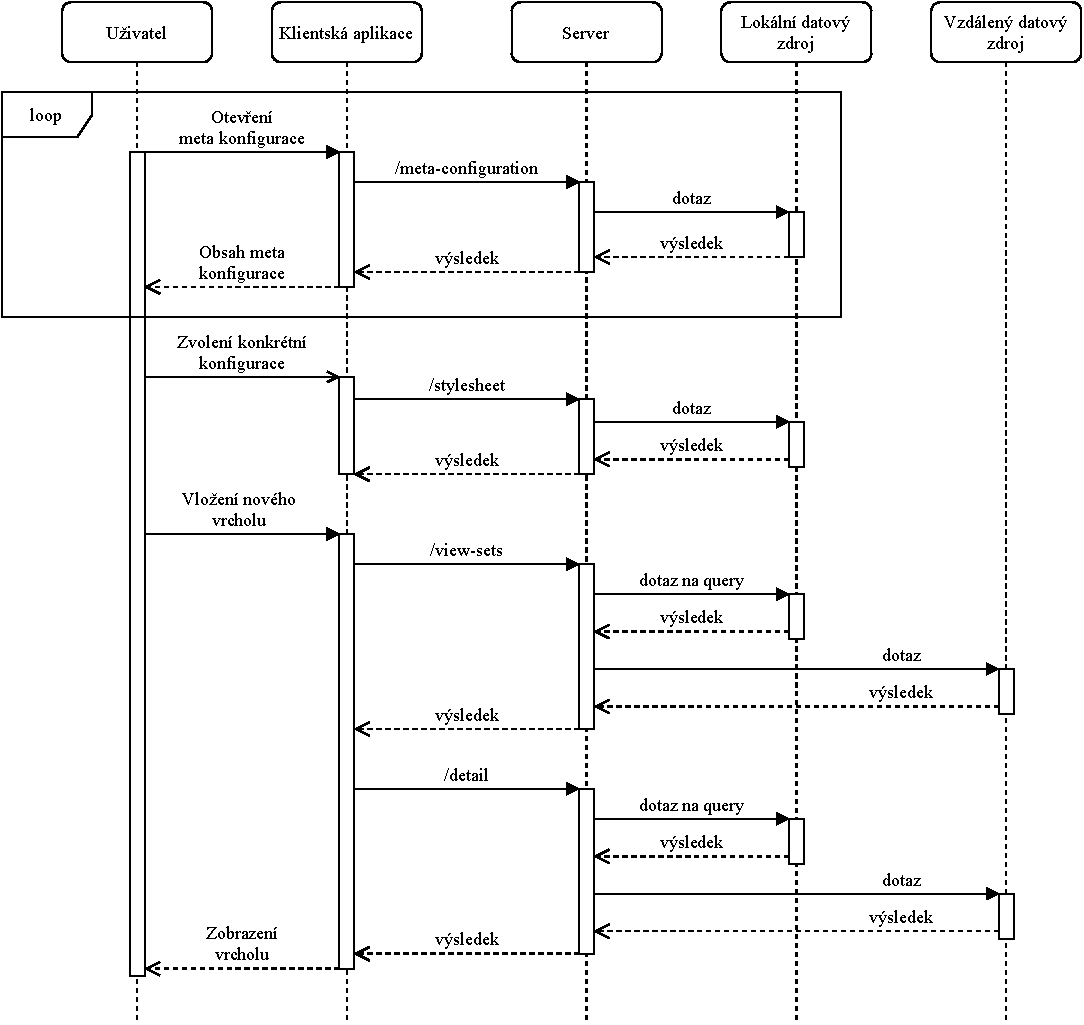
\includegraphics[width=\textwidth]{media/sequence-server.pdf}
    \caption{Schéma komunikace se serverem a RDF databází při spuštění aplikace. Nejprve klient vybírá konfiguraci. Poté začne stahování stylesheetu a stahování prvního vrcholu. Nejprve se stáhnout \texttt{view-sets} a poté z výchozího pohledu se stáhne \texttt{detail} a vrchol se zobrazí na grafu.}
\end{figure}


\section{Klient}

\begin{figure}
    \centering
    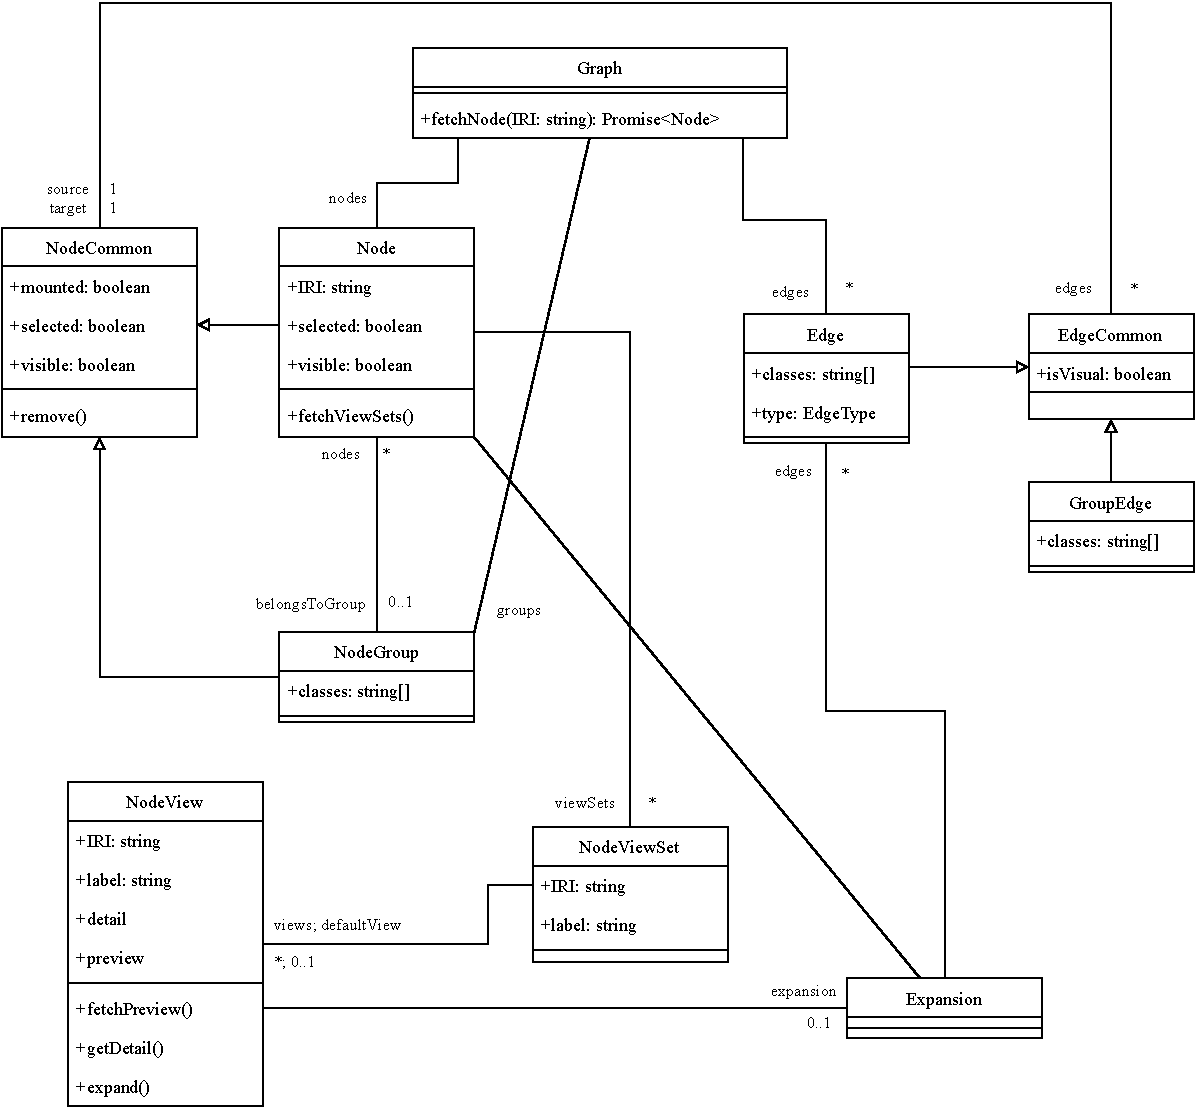
\includegraphics[width=\textwidth]{media/graph.pdf}
    \caption{Class diagram části aplikace jež pracuje s grafem.}
\end{figure}

\subsection{Moduly}

\subsubsection{Připojení na server}
Tento modul řeší komunikaci se serverem.

\subsubsection{Graf}
Tato část aplikace reprezentuje stažený graf a všechny jeho data. Má metody pro práci s grafem, jeho modifikaci a stahování nových dat ze serveru.

\subsubsection{Filtrování}
Tento modul integruje možnost filtrování vrcholů v aplikaci na základě různých grafových a sémantických vlastností. Modul se dá rozšířit o další filtry i za runtime a nabízí tedy možnost instalace pluginů.

\subsubsection{Layoutování}
Modul řeší uspořádání vrcholů v grafu. Layoutování reaguje na významné události z grafu. Jedná se například o vložení nového vrcholu, expanzi, přesunutí vrcholů, zamčení vrcholů atp. Stejně jako filtrování, jednotlivé layouty lze přidávat za runtime a je tedy možné s pomocí pluginů přidat nové layouty.

\subsubsection{Vyhledávání}
Modul vyhledávání vrací vrcholy na základě textového řetězce. Vyhledává v grafu, z autocomplete nebo se pokusí IRI sestavit z hledaného výrazu. Jednotlivé vyhledávače lze rozšířit o další stejně jako u filtrování a layoutování.

\subsubsection{Ukládání do souboru}
Řeší jak uložit a znova načíst stav aplikace do a ze souboru.
\chapter{Implementace}

\section{Vue.js framework}
Klientská část aplikace je postavena nad Vue.js frameworkem\footnote{\url{https://vuejs.org/}, \citet*{Vue}}, jež je populární JavaScriptový framework na stavbu uživatelských rozhraní. Protože některé z jeho funkcionalit byly použity v klíčových částech aplikace, je nutné čtenáře obeznámit alespoň se základním principem fungování frameworku.

\subsection{Vuex}
Vue.js framework, podobně jako konkurenční React\footnote{\url{https://reactjs.org/}} (Facebook) nebo Angular\footnote{\url{https://angularjs.org/}} (Google), využívají principu sledování stavu aplikace (jejich dat) pro automatickou změnu DOMu webové stránky. V praxi to znamená, že programátor může velice snadno napsat kód, který generuje uživatelské rozhraní na základě dat, která mohou být libovolně měněna bez nutnosti řešit problém, zda ke změně vůbec došlo a které části aplikace mají být o změně stavu informovány. Ve Vue tuto funkcionalitu zastává právě Vuex\footnote{\url{https://vuex.vuejs.org/}}, jež je možný používat samostatně.

Vuex drží stav aplikace jako jeden objekt, tedy slouží jako centrální úložiště dat pro celou aplikaci. Tento objekt se nazývá \textbf{store}. Změny ve storu mohou být sledovány Vuexem pro vykonání libovolných akcí, například překreslení textu na stránce, jež byl vykreslen Vue frameworkem.

\newcommand{\inlinecode}{\texttt}

Vrátíme-li se k původnímu příkladu, programátorovi stačí přiřadit do proměnné, jež je spravovaná Vuexem, novou hodnotu a Vuex se postará o zavolání všech komponent, které tuto proměnnou využívají a tyto komponenty na stránce překreslí původní hodnotu na novou. Překreslení přitom proběhne až poté, co skončí průběh aktuální funkce. Tohoto je docíleno pomocí \\  \texttt{Window.requestAnimationFrame()}. Díky tomuto můžeme stav v rámci průběhu jedné funkce modifikovat vícekrát se skoro nulovým dopadem na celkový výkon aplikace.

\subsubsection{Computed properties}

Kromě této funkcionality Vuex nabízí takzvané \textbf{gettery}, jež jsou ve Vue frameworku nazývány jako \textbf{computed properties}. Jedná se o funkce, které využívají data ze storu pro výpočet dat nových. Výhoda takovýchto getterů je ta, že Vuex dokáže výsledky těchto funkcí cachovat a přepočítává je pouze tehdy, změní-li se data původní. Interně gettery fungují tak, že při zavolání klientské funkce Vuex sleduje, které části storu byly dotázány a ty pak sleduje na změnu jež invaliduje cache konkrétního getteru. Při příštím požadavku na hodnotu se pak klientská funkce volá znovu a celá operace se opakuje.

Tyto computed properties jsou v aplikaci využívány často. Kupříkladu funkce, která počítá, zda je sousední vrchol vybrán. Na takovouto hodnotu se v aplikaci můžeme ptát libovolně krát, ale počítá se pouze tehdy, když se množina sousedních vrcholů vrcholu změní, nebo se změní právě označení vrcholu z množiny.

\subsubsection{Watchers}

Ve Vue lze využívat i \textbf{watch}ery, které umožňují registraci callbacku na změnu určité proměnné ve stavu. Watchery má smysl využívat tam, kde již data přestávají být spravována Vue frameworkem, tedy u knihoven třetích stran. Watchery, podobně jako překreslení komponent, jsou volány až po skončení probíhající funkce.

\subsubsection{Změna stavu}

Jak již bylo zmíněno, stav lze měnit přiřazením do proměnné, popřípadě voláním metod jako \texttt{.push()} na poli. Vuex dokáže tyto změny sledovat nahrazením původní proměnné (máme na mysli položku objektu) JavaScriptovým setterem. U polí dojde k obalení metody \texttt{.push()}, jež registruje změnu stavu.

Tento přístup má několik nevýhod, které se promítly i při vývoji klientské aplikace:
\begin{itemize}
  \item Vue není plně kompatibilní s novými \textbf{ES6 kontejnery} \texttt{Map} a \texttt{Set} a proto jsou v aplikaci používány jen v rámci lokálních proměnných a mapa je nahrazena klasickým objektem.
  \item Protože je v JavaScriptu nemožné sledovat \textbf{vytvoření nové property objektu}, musí programátor v tomto případě volat ručně \texttt{Vue.set(target, propertyName/index, value)} a \texttt{Vue.delete}, popřípadě vytvořit nový objekt, který nahradí ten původní.
  \item Je důležité mít na paměti, že data ve storu již nejsou původními objekty v pravém slova smyslu, protože veškeré fieldy a metody u objektů a polí byly nahrazeny, jak je zmíněno výše. Proto předání objektů a polí ze storu knihovnám třetích stran je nutné ošetřit \textbf{klonováním objektu}, jinak může dojít k zaseknutí aplikace.
  \item Instance tříd \textbf{knihoven třetích stran může zaseknout aplikaci}, pokud ji uložíme do storu. Bohužel, tohoto je velmi snadné ve Vue frameworku dosáhnout omylem.

  Řešením je využití problému, jež je popsán ve druhém bodě tohoto seznamu. (Ačkoli se může zdát, že se jedná o zneužití dokonalosti knihovny, je tento postup doporučován vývojáři frameworku.) Pokud chceme objektu nastavit kupříkladu instanci knihovny třetí strany, uložíme ji do \textbf{předem neinicializovaného} fieldu v metodě \texttt{mounted}. Taková proměnná pak nebude sledována a tedy nedojde k jejímu prohledání Vuexem.
\end{itemize}

\subsection{Vue framework}
Vue framework využívá takzvané komponenty. Komponentou se rozumí prvek na stránce, se kterým má smysl pracovat samostatně. Každá komponenta má vlastní HTML, CSS a JS. Komponenty se mohou do sebe zanořovat a vytvářet tak větší komponenty z menších. Příkladem může být komponenta \textit{seznam} jež dokáže na stránku vykreslit seznam prvků. Takováto komponenta by pak mohla mít podkomponenty jako \textit{prvek seznamu}.

Každé komponentě lze předat data formou \textbf{properties}, přičemž komponenta na základě těchto dat může vyrobit pod sebou další komponenty a předat jim část dat, která dostala.

Tato předávána data jsou právě data ze storu. Vue framework doporučuje, aby data, co komponenta dostane formou properties, neupravovala přímo, ale místo toho posílala události rodičovské komponentě, která data upraví. Ve své práci jsem se \textbf{rozhodl toto doporučení ignorovat}, neboť by tímto vzrostla náročnost na správu aplikace.

\begin{figure}[h]
    \centering
    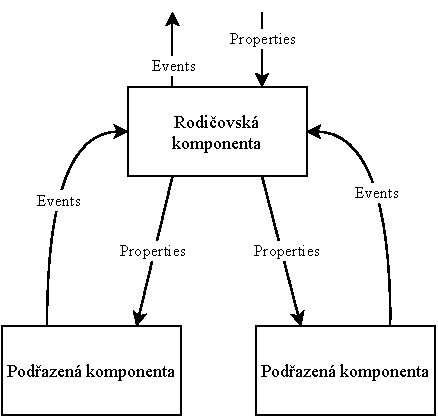
\includegraphics[width=0.5\textwidth]{media/vue.pdf}
    \caption{Doporučený způsob komunikace mezi komponentami ve Vue frameworku}
\end{figure}

\subsection{Mixins}
Někdy může být žádoucí, aby vícero komponent sdílelo stejnou množinu funkcí. V klasickém programování toto odpovídá dědičnosti tříd. Vue má takzvané Mixiny. Mixin je objekt, který komponentě dodává logiku navíc. Mixiny se dají použít jak v případě dědičnosti, kdy komponenty řeší podobný problém, tak i v případě, kdy kód jedné komponenty je příliš dlouhý a vyplatí se ho rozdělit na více částí. Mixiny totiž umožňují i vícenásobnou dědičnost.

\subsection{Loaders}
Kód Vue komponent se zapisuje do souborů s příponou \texttt{.vue}. Při sestavování aplikace se pak použije \texttt{vue-loader}, který ze souboru vyextrahuje zvlášť CSS, JS a HTML a ty předá dál na zpracování. HTML kód komponent není ve skutečnosti pravý HTML. Jedná se nadstavbu umožňující psát speciální značky, jež rozhodují kolikrát a jestli vůbec se tag na stránce vyrenderuje. Tato HTML nadstavba je pak předána \texttt{vue-template-compiler}, který vyrobí optimalizovaný JS kód jež renderuje HTML na základě stavu komponenty.

\newpage

\begin{prikl}
Ukázka jednoduché Vue komponenty \texttt{IndexedList}, která má parametr \texttt{list} očekávající pole stringů. Tato komponenta vypíše pole v odrážkovém seznamu ve formě \texttt{index: hodnota}. Komponenta se sama stará o překreslení DOMu, když se změní data. Komponentu můžeme v jiné komponentě použít vložením \texttt{<indexed-list :list="inputData" />}, kde \texttt{inputData} je proměnná obsahující pole stringů.

\begin{code}
<template>
  <ul>
    <li v-for="(item, index) in list" :key="index">
      {{index}}: {{ item }}
    </li>
  </ul>
</template>

<script lang="ts">
  import {Component, Prop} from "vue-property-decorator";
  import Vue from "vue";
  @Component
  export default class IndexedList extends Vue {
    @Prop() private list: string[];
  }
</script>

<style scoped lang="scss">
  ul {
    color: red;
  }
</style>
\end{code}
\end{prikl}

\subsubsection*{Scoped styly}

Můžeme si povšimnout \texttt{scoped} stylů v ukázce. Vue má mechanismus, že styly, které zde nastavíme, se aplikují jen na tuto komponentu. Nastavením červené barvy na seznam jsme tedy skutečně nastavili červenou barvu jen této komponentě a ostatní seznamy jsou netknuté. Toto má nespornou výhodu pokud pracujeme s velkým množstvím komponent a hrozilo by, že bychom museli používat složitě pojmenované css třídy, aby nedošlo ke kolizi.

Pokud bychom chtěli ovlivnit styly vnořených komponent a máme nastavené scoped styly, musíme použít pseudo selektor \texttt{::v-deep}, kupříkladu \\  \texttt{.actions ::v-deep .v-input--selection-controls}. Tohoto je hodně používáno, pokud je potřeba upravit styly Vuetify frameworku (viz dále).

\newpage






\section{Cytoscape knihovna}

Cytoscape.js\footnote{\url{https://js.cytoscape.org/}, \citet{10.1093/bioinformatics/btv557}} je JavaScriptová knihovna na kreslení grafů s pomocí technologie canvas\footnote{Canvas umožňuje kreslit bitmapové obrázky na stránku. Alternativou této technologie je SVG, která pracuje s vektorovými objekty. Její nevýhodou je, že pro větší grafy může limitovat výkon aplikace.}, která byla využita v tomto projektu.

Cytoscape umožňuje definovat graf pomocí vrcholů a hran, který bude vykreslen na obrazovku, kde může uživatel přesouvat jednotlivé jeho části, měnit přiblížení grafu, označovat vrcholy a podobně. Kromě toho podporuje širokou škálu možností, jak vizuálně obarvit vrcholy. Tato pravidla jsou dodávána jako style sheet a odpovídají těm, které byly zmíněné v kapitole \ref{pozadavky-visual-style-sheet}.

V knihovně lze zaregistrovat callbacky na různé události grafu a tímto jsme schopni na ně v aplikaci reagovat a propojit knihovnu i s Vue frameworkem. Umožňuje také měnit stav grafu průběžně a vytvářet tak animace, kupříkladu plynulé přiblížení grafu.

Cytoscape podporuje layoutování grafu s pomocí pluginů. V této práci byl využit Cola layout\footnote{\url{https://github.com/cytoscape/cytoscape.js-cola}}, který využívá fyzikální simulaci na esteticky příjemné uspořádání vrcholů. Původní plugin byl v mírně upraven, aby vyhovoval požadavkům na uzamykání pozic vrcholů. Kromě Coly je v aplikaci využit Dagre layout, který vrcholy uspořádá do stromové struktury.

\paragraph{Třídy} Cytoscape podporuje přidávání tříd vrcholům obdobně, jako třídy v HTML. Na tyto třídy je pak možné nastavit pravidla style sheetů. Toho je v aplikaci právě využito tak, že náhled (\ref{pozadavky-preview}) vrací seznam tříd, které budou nastaveny vrcholům a podle těchto tříd budou vrcholy barevně a jinak vizuálně rozlišeny.


\begin{prikl}
Ukázka kódu, který vytváří nový vrchol. Jak lze vidět, vytvářenému vrcholu nastavujeme ihned pozici a třídy. Kromě tříd může nést další data jako popisek (label), který se pak zobrazí jako text u vrcholu. Vrcholu jsou nastavena všechna data z \texttt{preview}, na které lze reagovat a používat je v rámci style sheetů.
\begin{code}
this.element = this.cy.add({
    group: 'nodes',
    data: {
      label: '-',
      ...clone(this.node.lastPreview),
      id: this.node.IRI
    },
    classes: this.classList,
    position,
});
\end{code}
Za povšimnutí stojí i funkce clone, která je nutná, neboť předáváme objekt z Vue frameworku.
\end{prikl}


\newpage

\section{Vuetify framework}
Na stavbu uživatelského rozhraní aplikace je pak využit Vuetify framework\footnote{\url{https://vuetifyjs.com/}}, jež je navržen pro spolupráci s Vue frameworkem. Obsahuje sadu předefinovaných komponent, které lze v aplikaci snadno použít a stavět z nich komponenty vlastní. Jedná se například o tlačítka, rozevírací seznamy, načítací lišty, dialogy, karty a další grafické prvky. Všechny komponenty Vuetify frameworku mají v názvu charakteristický prefix \texttt{v-}.

\section{Prostředí}
Klientská část aplikace je napsána v jazyce TypeScript\footnote{\url{https://www.typescriptlang.org/}}, což je typovaná nadstavba JavaScriptu. Projekt využívá balíčkovací nástroj npm\footnote{\url{https://www.npmjs.com/}} a je sestavován pomocí \texttt{@vue/cli-service}. Ten interně využívá Webpack\footnote{\url{https://webpack.js.org/}} pro sestavení celého projektu.

\subsection{Instalace}
Pro úspěšné přeložení aplikace je nutné vytvořit soubor \texttt{./conf.yaml}, který přepisuje nastavení ze souboru \texttt{./conf.default.yaml}. V tomto souboru lze nastavit výchozí jazyk aplikace, výchozí IRI meta konfigurace a URL adresu, kde se nachází server.

Pro přeložení projektu je pak nutné spustit
\begin{enumerate}
  \item \texttt{npm install} pro stažení a případnou aktualizaci balíčků, na kterých aplikace závisí.
  \item \texttt{npm run build} pro přeložení projektu.
\end{enumerate}

Výsledné soubory jsou umístěny v adresáři \texttt{./dist} včetně souboru \texttt{index.html}, odkud se aplikace spouští. Webový server by tedy měl odkazovat právě do tohoto adresáře.

\subsection*{Lokalizace aplikace}
Aplikaci lze přeložit do více světových jazyků přidáním souboru \\\texttt{<jazykový-kód>.yaml} do adresáře \texttt{./locales}. Soubor vytvořte jako kopii souboru \texttt{en.yaml}, jež obsahuje anglické překlady. Aplikaci pak stačí znova přeložit a vytvořený jazyk bude v aplikaci dostupný.

\newpage

\subsection{Adresářová struktura}
\dirtree{%
.1 /.
.2 dist \DTcomment{Adresář s vyrobenými .js a .css soubory. Obsahuje také výchozí index.html soubor.}.
.2 locales \DTcomment{Adresář s .yaml překlady aplikace.}.
.3 en.yaml \DTcomment{Anglický překlad a referenční soubor pro překlady do jiných jazyků.}.
.2 public \DTcomment{Adresář se statickými soubory.}.
.3 index.html \DTcomment{Šablona pro soubor index.html.}.
.2 src.
.3 @types \DTcomment{Definice typů pro knihovny, jež nemají oficiální typy pro Typescript.}.
.3 component \DTcomment{Obsahuje Vue komponenty.}.
.4 filter \DTcomment{Adresář s pomocnými komponentami pro filtry.}.
.4 graph \DTcomment{Adresář s komponentami pro práci s grafem.}.
.4 helper \DTcomment{Adresář s pomocnými komponentami, jež jsou použitelné v rámci celé aplikace.}.
.4 side-panel \DTcomment{Adresář s komponentami pro pravý boční panel.}.
.4 Application.vue \DTcomment{Top level Vue komponenta. Zde se vše registruje.}.
.3 configurations \DTcomment{Obsahuje logiku pro správu konfigurací a meta konfigurací.}.
.3 file-save \DTcomment{Interface pro třídy které obsahují uložitelná data.}.
.3 filter \DTcomment{Logika filtrování a jednotlivé filtry na skrývání vrcholů.}.
.4 filters \DTcomment{Obsahuje adresáře s jednotlivými filtry.}.
.3 graph \DTcomment{Třídy reprezentující lokální graf.}.
.3 layout \DTcomment{Logika layoutů.}.
.4 layouts \DTcomment{Obsahuje adresáře s jednotlivými layouty.}.
.3 remote-server \DTcomment{Třídy pro stahování dat ze vzdáleného serveru.}.
.3 searcher \DTcomment{Logika vyhledávání.}.
.4 searchers \DTcomment{Obsahuje jednotlivé vyhledávače.}.
.3 LiteralTranslator.ts \DTcomment{Pomocná metody pro překlad.}.
.3 conf.ts \DTcomment{Pomocný export soubor pro konfiguraci.}.
.3 i18n.ts \DTcomment{Inicializuje překlad aplikace.}.
.3 main.ts \DTcomment{Počáteční soubor aplikace.}.
.2 conf.default.yaml \DTcomment{Výchozí nastavení aplikace.}.
.2 conf.yaml \DTcomment{Uživatelem předefinované nastavení aplikace.}.
.2 package.json \DTcomment{Balíčky pro NPM. Obsahuje seznam závislostí aplikace.}.
.2 tsconfig.json \DTcomment{Konfigurační soubor pro Typescript.}.
.2 vue.config.js \DTcomment{Konfigurační soubor pro balíčky aplikace.}.
}

\newpage


\section{Programátorská dokumentace}
V této sekci budou postupně rozebrány klíčové třídy a komponenty aplikace.

\subsection{Vstupní skript a pomocné soubory}
Vstupním skriptem celé aplikace je soubor \texttt{main.ts}, ve kterém je inicializován Vuetify a Vue framework, který spouští komponentu Application, jež je výchozí komponentou celé aplikace.

V tomto souboru je také includován soubor \texttt{LiteralTranslator.ts}, který přidává pomocné globální metody (v rámci Vue frameworku jsou dostupné pod \texttt{this}) pro překlad literálů z grafu.

\begin{itemize}
  \item \texttt{\$t_literal(translations): string|undefined} - Očekává objekt \\popsaný v kapitole \ref{jazykova-podpora} a vybere z něj nejvhodnější překlad podle pravidel popsaných ve zmíněné kapitole. Vrací \texttt{null}, pokud žádný překlad není.

  \item \texttt{\$te_literal(translations): boolean} - Vrací true, pokud by předchozí metoda našla překlad.

  \item \texttt{\$i18nGetAllLanguages(): string[]} - Vrací jazyky, které jsou požadovány ze serveru. Pokud se jazyk aplikace změní a na již stažená data vrátí \texttt{\$te_literal} false, pak se data stáhnou znovu s již správným jazykem. Tato logika je zatím implementována pouze u meta konfigurací a konfigurací.
\end{itemize}

\subsection{Komponenta Application}\label{komponenta-application}
Jedná se kořenovou komponentu celé aplikace, která drží základní třídy a moduly a řídí logiku celé aplikace. Tato komponenta registruje veškeré dialogová okna a grafické prvky.

Pro debugování aplikace je komponenta přístupná pod \texttt{window.kgvb} a je tedy možné zasahovat do jakékoli části aplikace.

Mezi důležité fieldy patří (veškeré tyto třídy budou popsány dále v textu):
\begin{itemize}
  \item \texttt{server: RemoteServer} - Třída komunikující se serverem. Obsahuje metody, které zavolají na serveru konkrétní požadavek a vrátí výsledek ve správném interface nebo false, pokud nastala chyba.
  \item \texttt{configuration: Configuration} - Aktuální konfigurace grafu ve smyslu konfigurace z kapitoly \ref{pozadavky-konfigurace}.
  \item \texttt{graph: Graph} - Aktuální graf jež závisí na \texttt{configuration}.
  \item \texttt{areaManipulator: GraphAreaManipulator} - Třída, která obsahuje \\ metody pro práci s grafovou oblastí jako přibližování, přesouvání pohledu atp.
  \item \texttt{manipulator: GraphManipulator} - Třída, která obsahuje metody pro složitější práci s grafem. Na rozdíl od \texttt{Graph}, metody v této třídě více odpovídají akcím uživatele a obvykle volají další moduly jako \texttt{LayoutManager}.
  \item \texttt{viewOptions: ViewOptions} - Jednoduchá třída mající stav, jak pohlížet na graf. Řeší, zda u hran mají být popisky a zda vůbec mají být hrany viditelné. U vrcholů pak řeší také viditelnost popisků a zda se mají zobrazit jako malé tečky.
  \item \texttt{filter: FiltersList} - Modul řešící filtrování.
  \item \texttt{layouts: LayoutManager} - Modul řešící layoutování grafu v závislosti na určitých akcích uživatele.
  \item \texttt{configurationManager: ConfigurationManager} - Drží všechny načtené konfigurace a meta konfigurace ze serveru.
  \item \texttt{visualStyleSheet: ResponseStylesheet} - Aktuální style sheet pro \\ Cytoscape knihovnu.
  \item \texttt{graphSearcher: GraphSearcher} - Třída schopna vyhledávat vrcholy v grafu a z autocomplete souborů, jež jsou specifikovány v konfiguraci.
\end{itemize}

\begin{figure}[h]
    \centering
    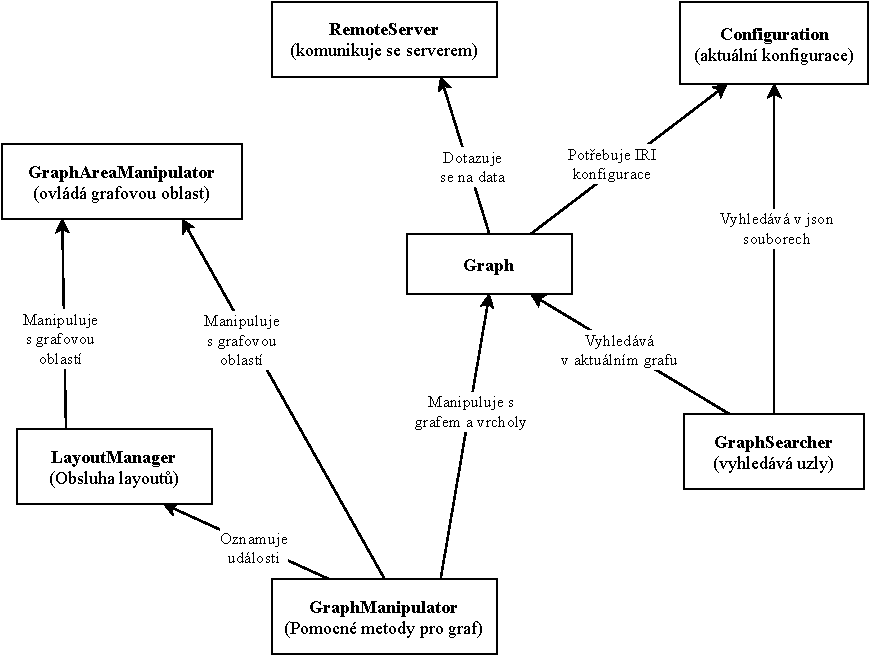
\includegraphics[width=0.8\textwidth]{media/dependencies.pdf}
    \caption{Závislosti jednotlivých tříd aplikace na sobě. Tato závislost přibližně odpovídá závislosti modulů znázorněné na obrázku \ref{fig:module-dependencies}.}

\end{figure}

\subsubsection{Závislost modulů}

Značná část modulů v aplikaci je závislá na jiných. Kupříkladu \texttt{Graph} je závislý na \texttt{RemoteServer} a částečně na \texttt{Configuration}. Na třídě \texttt{Graph} pak závisí \texttt{GraphAreaManipulator} na které závisí \texttt{GraphManipulator}. Protože těchto závislostí je hodně, některé třídy byly určeny jako readonly a tedy se může měnit pouze jejich stav. Jedná se například o třídu \texttt{RemoteServer} které lze měnit URL adresu serveru. Dalšími třídami jsou \texttt{GraphAreaManipulator}, \texttt{ViewOptions}, \texttt{FiltersList}, \texttt{LayoutManager}, \texttt{ConfigurationManager}. Ostatní třídy jsou pak měněny pouze když se mění konfigurace, v tu chvíli se starý graf zahazuje a vytváří se nový.

\medskip

Mezi důležité metody patří
\begin{itemize}
  \item \texttt{async loadStylesheet()} - Načte style sheet do proměnné \\ \texttt{visualStyleSheet} podle aktuální konfigurace \texttt{configuration}.
  \item \texttt{changeConfiguration()} - Nastaví novou konfiguraci \texttt{configuration} a zavolá metodu \texttt{createNewGraph}.
  \item \texttt{createNewGraph(loadStylesheet: boolean = true)} - Na základě konfigurace \texttt{configuration} vytvoří nový, prázdný graf (startý zahodí) a nastaví závislosti mezi moduly. Tato metoda pak ještě resetuje nastavení filtrů a plátna kde se vykresluje graf.
  \item \texttt{updateGraphSearcher()} - Pomocná metoda pro \texttt{createNewGraph}, která na základě konfigurace a grafu sestaví třídu schopnou vyhledávat nové vrcholy v grafu.
\end{itemize}

Kromě těchto metod komponenta obsahuje ještě Vue metodu \texttt{mounted}, která skryje uvítací obrazovku aplikace, až se komponenta (a tedy i celá aplikace) inicializuje. Kontroluje také URL adresu, zda neobsahuje parametry \texttt{load}, \\ \texttt{meta-configuration} nebo \texttt{configuration} které přimějí aplikaci načíst graf z url, respektive načíst meta konfiguraci, respektive konfiguraci.

\subsubsection{ApplicationLoadStoreMixin}
\texttt{ApplicationLoadStoreMixin} rozšiřuje komponentu o načítání a ukládání grafu ze a do souboru.

\paragraph{askForSaveAndPerformAction(modal: boolean, callback: Function)}\mbox{}\\ Tato funkce zkontroluje, zda jsou v grafu nějaké neuložené změny a pokud ano, otevře \texttt{SaveDialog} komponentu. Podle odpovědi na dialog pak graf uloží a v případě kladného potvrzení zavolá \texttt{callback} funkci, která pak může například vytvořit nový graf. Pokud žádné změny nejsou, callback je volán okamžitě.

\paragraph{loadFromFile(file: File), loadFromUrl(url: string)} - Metoda otevře soubor, respektive soubor z URL a přečte ho jako JSON. Výsledný objekt pak předá metodě \texttt{ObjectSave::restoreFromObject}.

\paragraph{saveToFile()} - Vyrobí soubor se stavem aplikace který je možné stáhnout.

\subsection{Interface ObjectSave}
Interface \texttt{ObjectSave} předepisuje dvě metody \texttt{saveToObject(): object} a \texttt{restoreFromObject(object: any): void}, které uloží stav třídy do serializovatelného objektu, respektive tento stav obnoví. Tento interface obsahují všechny třídy jež drží stav aplikace který je třeba uložit do souboru, pokud o to uživatel požádá.

Tento interface implementuje i komponenta \texttt{Application} jež tyto metody volá na modulech a jednotlivé výsledky pak spojí do jednoho objektu (v případě metody \texttt{saveToObject}). Výsledek je pak serializován do JSONu a uložen do počítače. V opačném případě je JSON deserializován a předán metodě \texttt{restoreFromObject} která volá tuto metodu na modulech, které ji mohou volat na podtřídách.

\paragraph{Poznámka:} Je třeba mít na paměti, že metoda \texttt{saveToObject} by měla vracet plain Javascript objekt, tedy veškeré neprimitivní typy, jako objekty a pole musí být klonovány, pokud jsou ve vlastnictví Vue frameworku. Taktéž je třeba dbát na zpětnou kompatibilitu u metody \texttt{restoreFromObject}.

\smallskip

Do budoucna se nabízí tento interface rozšířit o více módů ukládání. Tento problém je popsán v poslední kapitole.

\subsection{Třída Graph}

\begin{figure}
    \centering
    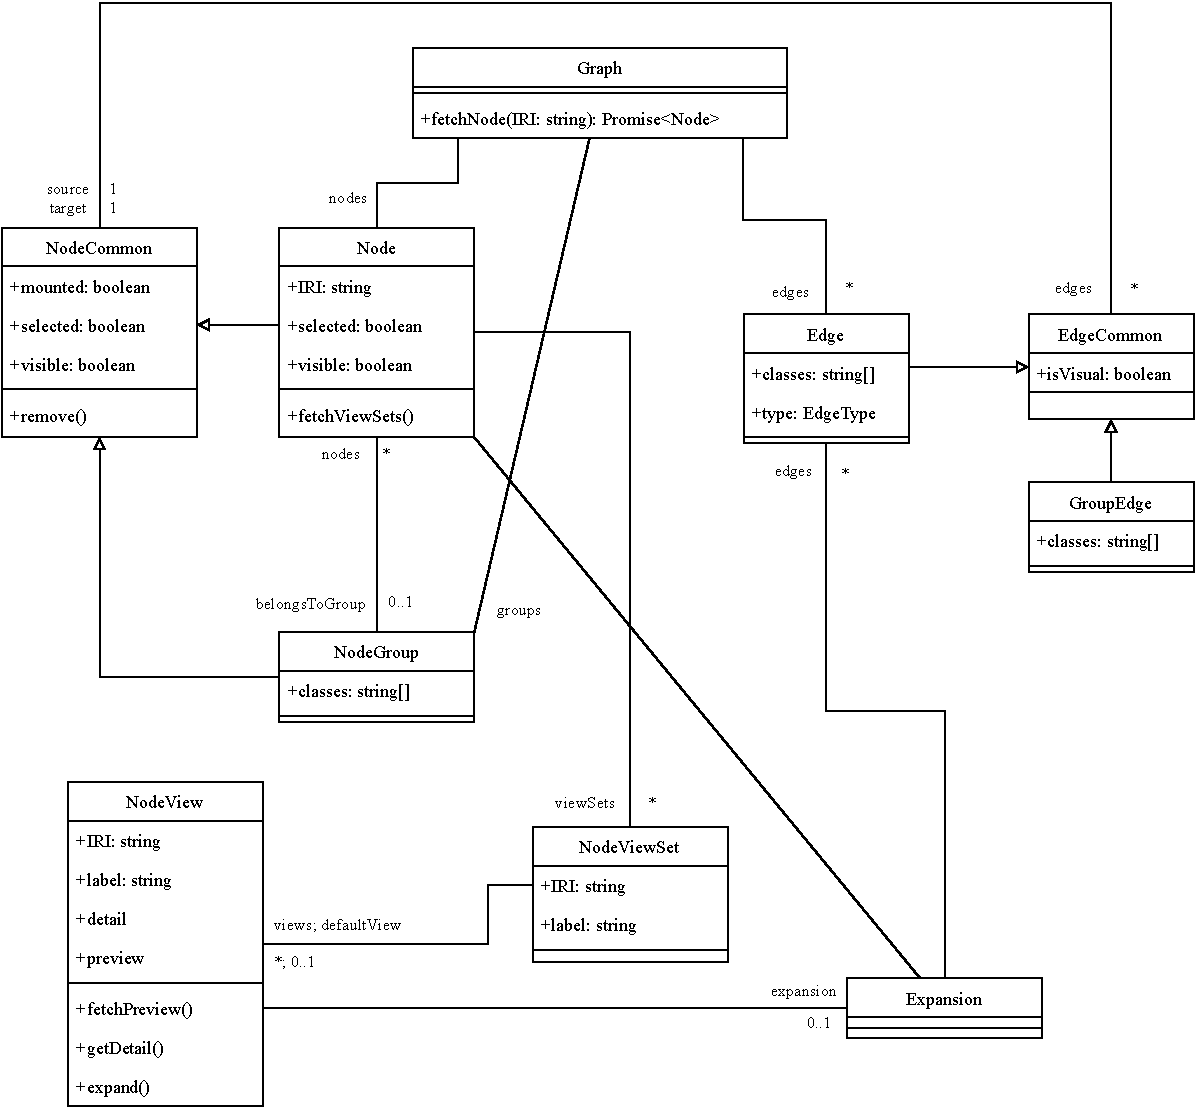
\includegraphics[width=\textwidth]{media/graph.pdf}
    \caption{Class diagram tříd, které pracují s grafem.}
\end{figure}

Třída \texttt{Graph} umístěna v \texttt{graph/} spravuje stažený graf pod konkrétní konfigurací. Závisí na \texttt{server: RemoteServer} a \texttt{configuration: Configuration}. Pokud se konfigurace mění, nebo se načítá nový graf ze souboru, je tato třída zahozena. Ačkoli třídy jako \texttt{Node} nebo \texttt{Edge} obsahují fieldy pro obsluhu viditelného grafu, třída \texttt{Graph} a ostatní nemusí být explicitně použity na vykreslení grafu na plátno, ale mohou být použity pro držení obecného grafu.

\subsubsection*{Fieldy}
\begin{itemize}
  \item \texttt{nodes} objekt tříd \texttt{Node} - Seznam všech vrcholů grafu.
  \item \texttt{edges} objekt tříd \texttt{Edge} - Seznam všech hran stažených ze serveru.
  \item \texttt{groups: NodeGroup[]} - Seznam všech neprázdných skupin vrcholů.
  \item \texttt{nodesVisual: NodeCommon[]} - Všechny \texttt{Node} a \texttt{NodeGroup}, které jsou aktuálně viditelné v grafu. \textit{Viditelnost vrcholů je popsána dále.}
  \item \texttt{groupEdges: GroupEdge[]} - Hrany které propojují skupiny vrcholů nebo skupinu a normální vrchol. Tyto hrany vznikly sloučením několika hran a existují pouze díky existenci nějaké skupiny vrcholů.
  \item \texttt{edgesVisual: EdgeCommon[]} - Všechny \texttt{Edge} a \texttt{GroupEdge} které jsou aktuálně viditelné v grafu. \textit{Viditelnost hran je popsána dále.}
\end{itemize}

Poslední tři zmíněné fieldy jsou gettery. Protože se aplikace často na tyto proměnné dotazuje, je využito Vuexu a tyto hodnoty jsou ve skutečnosti computed properties. Protože třída \texttt{Graph} není komponentou, má také field \texttt{vuexComponent: GraphVuex} na komponentu, která se vytvoří automaticky společně s grafem a tyto zmíněné fieldy počítá. Tak docílíme cachování těchto hodnot a k jejich přepočítání dojde pouze tehdy, změní-li se hrany, nebo vrcholy v grafu.

\subsubsection*{Metody}
\begin{itemize}
  \item \texttt{getNodeByIRI(IRI: string): Node|null} - Vrátí vrchol dle jeho IRI nebo \texttt{null} v případě, že neexistuje.

  \item \texttt{createNode(IRI: string): Node} - Vytvoří a zaregistruje nový vrchol v grafu.
  \item \texttt{createEdge(source: Node, target: Node, type: EdgeType): Edge}\mbox{}\\Vytvoří a zaregistruje novou hranu v grafu.
  \item \texttt{createGroup(): NodeGroup} - Vytvoří a zaregistruje prázdnou skupinu vrcholů.

  \item \texttt{getAllTypes(): Set<NodeType>} a \texttt{getAllClasses(): Set<string>}\mbox{}\\Pomocné metody, které projdou všechny vrcholy v grafu a shromáždí jejich typy, respektive třídy. Těchto metod je využíváno při filtrování, protože nejsme schopni ze serveru získat kompletní množinu typů a tříd. Metody jsou volány, když uživatel otevře okno s možnostmi filtrů.

  \item \texttt{fetchNode(IRI: string): Promise<Node>} - Vrchol je definován pouze svým IRI a tedy pro vytvoření vrcholu se aplikace nemusí ničeho dotazovat serveru. Tato metoda kromě vytvoření takového vrcholu ještě stáhne jeho \texttt{view-sets}, zvolí výchozí pohled a stáhne \texttt{preview} vrcholu. V případě, že se nepodaří stáhnout tyto informace, pak podle požadavku na vložení vrcholu z \ref{pozadavky-uzivatelske}, vrchol do grafu nebude přidán a metoda vrátí null.

  \item \texttt{getOrCreateNode(IRI: string): Promise<Node>} - Obdobná metoda \\metodě výše. Pokud vrchol neexistuje, volá předchozí metodu. Pokud vrchol existuje, stáhne jeho \texttt{view-sets} a \texttt{preview} obdobně jako předchozí metoda a vrátí ho.
\end{itemize}

\paragraph{Poznámka k viditelnosti} Veškeré metody, které vytvářejí vrcholy, skupiny nebo hrany, tyto prvky nevytvoří viditelnými. Aby mohl být prvek viděn v grafu, musí mu být nastaven field \texttt{mounted = true}.

\subsection{Třída NodeCommon}
Třída \texttt{NodeCommon} je společným předkem pro třídy \texttt{Node} a \texttt{NodeGroup} a zaštiťuje především jejich vizuální vlastnosti.

\subsubsection*{Fieldy}
\begin{itemize}
  \item \texttt{mounted: boolean} - Určuje, zda má být vrchol viditelný v aplikaci. Na rozdíl od ostatních úrovní viditelností je tato myšlena tak, že vrchol, který má tuto hodnotu false, v grafu vůbec nefiguruje a není jej možné ani najít v jiných částech aplikace (například mezi skrytými vrcholy). Využití najde v případě, kdy server pošle více vrcholů než uživatel žádal, nebo ho lze použít v případě browsingu seznamem, který je popsán v poslední kapitole.

  \item \texttt{onMountPosition: [number, number]} - Pomocný field, který určuje, kde má být vrchol na plátně vykreslen, až bude nastaven na mounted. Souřadnice odpovídají souřadnicím používanými Cytoscape knihovnou.

  \item \texttt{visible: boolean} - Nastavuje uživatelskou viditelnost vrcholu. Uživatel se může rozhodnout ručně skrýt vrchol. Takový vrchol si pak zachovává svou pozici na plátně a je v seznamu mezi ostatními skrytými vrcholy.

  \item \texttt{get isVisible: boolean} - Pomocný getter, který určí, jestli je vrchol viditelný. Pro \texttt{NodeGroup} se počítá jako \texttt{visible} AND \uv{alespoň jeden vrchol skupiny je \texttt{isVisible}}.  \texttt{Node} pak viditelnost počítá jako \texttt{visible} AND \uv{žádný filtr nezakazuje jeho viditelnost}.

  \item \texttt{selected: boolean} - Pokud je vrchol vybrán, je zobrazen jeho detail v pravém panelu aplikace. Je možné vybrat více vrcholů. Vybrání vrcholů je napojeno na vybírání vrcholů na plátně. Lze vybrat i skryté vrcholy (uživatelem, nebo filtrem). Pokud vrchol není mounted, je tato hodnota ignorována.

  \item \texttt{get neighbourSelected: boolean} - Pomocný getter, který vrátí true, pokud sousední vrchol byl vybrán. Využívá se pro zvýraznění sousedních vrcholů vybraného vrcholu v grafu.

  \item \texttt{get identifier: string} - Jednoznačný identifikátor pro potřeby Cytoscape knihovny.

  \item \texttt{get selfOrGroup: NodeCommon} - Pomocný field, který vrátí buď sebe, nebo skupinu do které vrchol patří. Využití má čistě pro zjednodušení programování a využívá se například v částech kódu, kde se řeší kontrakce hran.

  \item \texttt{lockedForLayouts: boolean} - Pokud daný layout podporuje zamykání pozic vrcholů, tato proměnná určuje, jestli je jeho pozice zamčená.
\end{itemize}

\subsubsection*{Metody}
\begin{itemize}
  \item \texttt{remove()} - Smaže vrchol z grafu společně s jeho hranami. V případě skupiny smaže skupiny a vrcholy v ní.
  \item \texttt{selectExclusively()} - Nastaví \texttt{selected} pouze pro tento vrchol. V praxi to znamená, že se zobrazí detail tohoto vrcholu v pravém panelu.
\end{itemize}

\paragraph{Poznámka} Díky Vue frameworku je hodně akcí vyvoláno právě nastavením nějaké proměnné. Kupříkladu proměnná \texttt{mounted} místo metody \texttt{mount()}. Vue framework automaticky při změně takovýchto proměnných provede příslušnou akci. Tento přístup má několik výhod, kupříkladu můžeme napojit proměnnou \texttt{visible} na checkbox a tak propojit viditelnost vrcholu se zaškrtávacím políčkem v obou směrech. Nevýhoda tohoto přístupu je ta, že skutečná akce bude provedena až po skončení funkce. Pokud bychom například chtěli počkat, až se vrchol namountuje a pak provést nějakou akci, musíme počkat na další AnimationFrame. Následující kód toto předvádí na akci, kdy chceme vrchol zobrazit v grafu a pak na něj přesunout pohled.

\begin{code}
node.mounted = true;
await Vue.nextTick(); // Mounting function is called
this.area.fit(node)
\end{code}

\subsection{Třída Node}
Třída \texttt{Node} rozšiřuje třídu \texttt{NodeCommon} a reprezentuje vrchol získaný ze serveru, tedy entitu z RDF databáze.

\subsubsection*{Fieldy}
\begin{itemize}
  \item \texttt{get classes: string[]} - Seznam tříd z posledního kompletního pohledu. \textit{(viz dále)}
  \item \texttt{get edges: Edge[]} - Seznam hran příslušících vrcholu.
  \item \texttt{filters} jako objekt - Objekt jehož klíčem jsou identifikátory filtrů a hodnotou je \texttt{boolean}, zda konkrétní filtr povoluje viditelnost vrcholu. Objekt je aktualizován kdykoli se změní stav vrcholu, který daný filtr využívá, nebo se změní nastavení filtrů. Všechny hodnoty nastavené na \texttt{true} jsou nutnou podmínkou viditelnosti vrcholu.
  \item \texttt{get shownByFilters: boolean} - Zdali všechny hodnoty objektu výše jsou nastaveny na true.
  \item \texttt{currentView: NodeView} - Určuje aktuální pohled na vrchol.
  \item \texttt{lastFullView: NodeView | null} - Tato proměnná odkazuje na poslední pohled na vrchol, který měl kompletní \texttt{preview}. Změna pohledu je totiž okamžitá, ale změněný pohled ještě nemusí mít stažený \texttt{preview}. To by způsobilo zbytečné \uv{blikání} vrcholu v grafu, když by uživatel měnil jeho pohledy. Na krátkou chvíli by totiž neměl žádné třídy a tedy by se vypnuly jeho styly.
  \item \texttt{viewSets} jako objekt \texttt{NodeViewSet} - Seznam view setů. Pokud view sety ještě nebyly staženy, pak je hodnota tohoto fieldu rovna \texttt{null}.
  \item \texttt{belongsToGroup: NodeGroup | null} - Určuje, zda vrchol patří do skupiny. Pokud ano, pak nebude zobrazen na plátně.
\end{itemize}


\subsubsection*{Metody}
\begin{itemize}
  \item \texttt{async fetchViewSets(): Promise<void>} - Metoda asynchronně stáhne view sety. Tato metoda (společně s dalšími) je navržena tak, že druhým voláním nezahájí druhé stahování, ale vrátí existující Promise z prvního. Takto nedojde k zatížení serveru a datových zdrojů. Ukázka metody je zobrazena an obrázku \ref{fetchViewSets}.
  \item \texttt{async useDefaultView(): Promise<NodeView>} - Metoda stáhne pohledy a nastaví výchozí, v případě že vrchol nemá nastaven žádný pohled.
\end{itemize}

\paragraph{Poznámka} Aktuální interface serveru vrací při expanzi detail vrcholů. Detail formálně patří k pohledu ale v odpovědi ze serveru není určeno, o jaký pohled se jedná. Takový pohled je pak nastaven jako aktuální, ale při volání metody \texttt{useDefaultView} bude ignorován a přepsán.


\begin{figure}
\begin{code}
private fetchViewSetsPromise: Promise<void> = null;

async fetchViewSets(): Promise<void> {
    let asynchronouslyFetchViewSets = async () => {
        let result = await this.graph.server.getViewSets(...);

        if (result) {
            this.viewSets = ...;
        }
        this.fetchViewSetsPromise = null;
    }

    if (!this.viewSets) {
        if (!this.fetchViewSetsPromise) {
            this.fetchViewSetsPromise = asynchronouslyFetchViewSets();
        }

        return this.fetchViewSetsPromise;
    }
}
\end{code}
\label{fetchViewSets}
\caption{Příklad kódu na stažení view setů. Metoda má vevnitř další metodu která je volána pouze tehdy, neskončila-li předchozí Promise. Takto zařídíme pouze jeden požadavek na server současně.}
\end{figure}

\subsection{Třída NodeGroup}
Třída \texttt{NodeGroup} rozšiřuje třídu \texttt{NodeCommon} a reprezentuje skupinu vrcholů \texttt{Node}. Aktuálně není podporováno, aby skupina obsahovala další skupiny. Všechny pomocné metody pro manipulaci v rámci skupiny pak řeší přeskupování tak, že prvně vrcholy ze skupiny odstraní a vloží je do jiné.



\subsubsection*{Fieldy}
\begin{itemize}
  \item \texttt{get classes: string[]} - Vrátí průnik tříd všech vrcholů, které obsahuje. Takto lze docílit, že skupina podobných vrcholů bude mít stejný styl jako jednotlivé vrcholy.
\end{itemize}

\subsubsection*{Metody}
\begin{itemize}
  \item \texttt{addNode(node: Node, overrideExistingGroup: boolean = false)}\mbox{}\\Vloží vrchol do skupiny.
  \item \texttt{checkForNodes()} - Pomocná metoda pro kontrolu, zda skupina vůbec nějaké vrcholy obsahuje. Pokud tomu tak není, odstraní se. Pokud obsahuje jen jeden vrchol, odstraní se a vrchol odstraní ze skupiny.
  \paragraph{Poznámka} Tato operace ve skutečnosti může být kontrolována Vue frameworkem. Nicméně kvůli jednoduchosti ruční implementace je vytváření a odstraňování skupin spravováno mimo framework.
\end{itemize}

\subsubsection{Generování GroupEdges}
\texttt{NodeGroup} seskupuje několik vrcholů a z grafového hlediska provádí jejich kontrakci. To znamená, že musíme sjednotit několik hran do jedné.

Třída obsahuje field \texttt{groupEdgesCache}, který udržuje tyto virtuální hrany. Kdykoli dojde ke změně v grafu, dojde k opětovnému přepočítání těchto virtuálních hran a pokud již existují, budou použity tyto existující. Pokud vznikne nová hrana, bude uložena do této cache a pokud nějaká hrana zanikla, bude z této cache odstraněna.

Tímto způsobem je docíleno automatického generování těchto hran, přičemž existující hrany se nemění (jejich instance zůstává stejná). Celý proces je spravován Vue frameworkem a tedy se děje automaticky.

Třída má field \texttt{get visibleGroupEdges: GroupEdge[]}, který vrací všechny hrany kromě těch, které vycházejí z jiné \texttt{NodeGroup}. Jednoduchým sjednocením pak dostaneme všechny hrany a každou právě jednou. Hrany se vypočítávají funkcí \texttt{getGroupEdgesInDirection}, která kvůli komplexnosti počítá hrany jen v jednom směru a musí se tedy volat dvakrát. Jak již bylo zmíněno, tato funkce používá cache, aby vracela již existující hrany. Výsledek funkce je pak ještě jednou cachován, tentokrát pomocí computed properties a tedy k přepočítání dojde pouze tehdy, změní-li se graf.

\subsection{Třídy EdgeCommon, Edge, GroupEdge}
Hrany RDF grafu jsou pak reprezentovány třídou \texttt{Edge} a hrany mezi skupinou a vrcholem, nebo dvěma skupinami třídou \texttt{GroupEdge}.

Společný předek předepisuje \texttt{get isVisual: boolean} který určuje, zda je hrana přítomná na plátně. Hrana je \texttt{isVisual} pokud její oba vrcholy jsou \texttt{mounted} a nepatří do skupiny. Obdobně pro \texttt{GroupEdge} je podmínka splněna pokud jsou oba vrcholy \texttt{mounted}.

\subsubsection*{Fieldy třídy Edge}
\begin{itemize}
  \item \texttt{type: EdgeType} - Typ hrany který určuje její label.
  \item \texttt{classes: string[]} - Třídy hrany.
\end{itemize}

\subsection{Třída NodeViewSet}
Třída reprezentuje view set popsaný v kapitole \ref{pozadavky-view-sets}. Jedná se o kontejner pro pohledy. Z hlediska implementace je třída velmi jednoduchá. Obsahuje seznam pohledů jako \texttt{views} a výchozí pohled \texttt{defaultView: NodeView}.

Obsahuje metodu \texttt{createView(IRI: string): NodeView}, která vytvoří \\a vhodně zaregistruje nový pohled. Protože jednotlivé pohledy jsou součástí jednoho požadavku (server na \texttt{view-sets} vrátí i pohledy) je logika vytváření pohledů ve třídě \texttt{Node}.

\subsection{Třída NodeView}
Tato třída odpovídá pohledům tak, jak jsou definovány v kapitole \ref{pozadavky-view}.

\subsubsection*{Fieldy}
\begin{itemize}
  \item \texttt{detail: DetailValue[]} - Představuje pole detailů, které lze získat ze serveru voláním \texttt{detail} a odpovídají \ref{pozadavky-detail}. Interface \texttt{DetailValue} pak obsahuje \texttt{type}, \texttt{IRI} a \texttt{value}. Aktuálně je \texttt{value} v rámci aplikace považována za textový řetězec. Do budoucna je možné aplikaci rozšít o více typů. Tomuto tématu se opět věnuje poslední kapitola.
  \item \texttt{preview: NodePreview} - Obsahuje základní informace o vrcholu, které řídí jeho vykreslení na obrazovce. Preview lze získat voláním \texttt{preview} na serveru a odpovídá definici v \ref{pozadavky-preview}.
  \item \texttt{expansion: Expansion} - Expanze dle tohoto pohledu. \textit{Třída je popsána dále.}
\end{itemize}

\subsubsection*{Metody}
\begin{itemize}
  \item \texttt{async getDetail(): Promise<DetailValue[]>} - Stáhne, uloží a vrátí detail.
  \item \texttt{async fetchPreview(): Promise<NodePreview>} - Stáhne, uloží a vrátí preview.
  \item \texttt{async expand(): Promise<Expansion>} - Provede expanzi a vrátí ji.
\end{itemize}

Všechny tři funkce mají podobnou ochranu proti opětovnému volání, jako metoda \texttt{fetchViewSets}, jejíž ukázka je na obrázku \ref{fetchViewSets}. Metoda \texttt{expand} používá třídu \texttt{Graph}, vytváří nové vrcholy a nastavuje jim \texttt{preview}. Nově vytvořené vrcholy nemají nastavené \texttt{mounted}, takže je lze snadno rozeznat a vhodně layoutovat.

\subsection{Třída Expansion}
Aktuálně třída \texttt{Expansion} je v aplikaci využívána pouze během procesu expanze. Do budoucna ji lze použít například pro znázornění vrcholů, které vznikly z jiných vrcholů v rámci expanze. Obsahuje seznam vrcholů \texttt{nodes: Node[]} a hran \texttt{edges: Edge[]}

\bigskip

Veškeré třídy zde zmíněné pro práci s grafem implementují rozhraní \\\texttt{ObjectSave} a tedy je možné na třídě \texttt{Graph} volat metody pro uložení a obnovení stavu.







\newpage

V následujících kapitolách práce bude popsáno, jak je tento modul grafu integrován do Vue frameworku tak, aby se samy vytvářely a aktualizovaly vrcholy a hrany, kdykoli dojde k jejich změně.

\subsection{Komponenta GraphArea} \label{komponenta-graph-area}
Tato komponenta je definována v souboru \\\texttt{src/component/graph/GraphArea.vue} a reprezentuje právě plátno, na které se vykresluje graf. Kromě plátna ještě vyrábí tlačítka v pravém dolním rohu na jeho ovládání a vyhledávací políčko v levém horním rohu.

Komponenta přijímá spoustu properties, nejdůležitější jsou však \\\texttt{graph: Graph} a \texttt{stylesheet: ResponseStylesheet}. Jakmile se komponenta vyrobí, vrátí rodičovské komponentě \texttt{Application} instanci třídy \\\texttt{GraphAreaManipulator} formou Vue emitu, jež je schopna pracovat právě s grafovou oblastí.

\subsubsection{GraphAreaStylesheetMixin}

Komponenta používá \texttt{GraphAreaStylesheetMixin} kde je oddělena logika \\zpracování style sheetů.

Předtím, než jsou styly předány Cytoscape knihovně, jsou použity výchozí styly z \texttt{defaultStyles}, které nastavují základní parametry. Poté jsou aplikovány styly, které komponenta dostala od rodiče a ten si je stáhl ze serveru. Nakonec jsou použity styly z \texttt{viewOptionsStyles}, které na základě \texttt{ViewOptions} přepisují základní pravidla.

Pokud se například rozhodneme v aplikaci skrýt hrany, právě poslední pravidlo je skryje.

Tato logika je sestavena v getteru \texttt{get finalStylesheet}, kde jsou ještě přidány pomocné styly jako \texttt{:selected}. (Jedná se o styly, které určují, jak bude vrchol zvýrazněn, když bude vybrán a další pomocné styly pro skrývání a animaci vrcholů.) Nakonec je použit watcher, který tuto proměnnou sleduje a když dojde ke změně, předá tyto styly Cytoscape knihovně. Logika této funkce je v následujícím kódu
\begin{code}
@Watch('finalStylesheet')
protected stylesheetUpdated() {
    this.cy.style(clone(this.finalStylesheet));
}
\end{code}
S pomocí dekorátoru nastavíme sledování \texttt{finalStylesheet}. Jakmile dojde k jeho změně, zavolá se metoda, která předá knihovně (\texttt{this.cy}) nový style sheet. Nesmíme zapomenout objekt klonovat, protože nemáme zaručeno, že ho knihovna nebude upravovat. Pokud by knihovna objekt vždy upravila, například z optimalizačních důvodů, Vue framework by zachytil změnu stylu a znovu by zavolal tuto funkci.

\newpage
Komponenta pak ke každému vrcholu, hraně a skupině vytvoří vlastní podkomponentu, která tento prvek reprezentuje a spravuje. Jako příklad uveďme vytvoření komponent reprezentujících vrchol.

\begin{code}
<graph-element-node
  v-for="node in graph.nodes"
  v-if="node.mounted && !node.belongsToGroup"
  :node="node"

  ...
/>
\end{code}

\bigskip

Mezi tlačítky v pravém dolním rohu se vykreslí i tlačítka aktuálního layoutu, pokud to daný layout podporuje. Layout v takovém případě musí dodat právě komponentu, která se zde vloží. V následujícím kódu se ověří, zda \texttt{buttons} není prázdné a použije se jako komponenta. Té je pak předán jeden parametr, a to aktuální layout.

\begin{code}
<component
  v-if="layoutManager.currentLayoutData.buttons"
  :is="layoutManager.currentLayoutData.buttons"
  :layout="layoutManager.currentLayout" />
\end{code}

\subsection{Komponenty GraphElementNode, GraphElementNodeGroup a GraphElementNodeMixin}
Jak již bylo zmíněno v popisu Vue frameworku a z příkladu výše, framework automaticky pro kažý vrchol grafu, který je \texttt{mounted} a není ve skupině, vytvoří komponentu \texttt{GraphElementNode}. Ta se pak stará o zobrazení tohoto vrcholu v rámci Cytoscape knihovny.

Obdobně jako jsme měli třídy \texttt{NodeCommon}, \texttt{Node} a \texttt{NodeGroup} i zde máme komponenty \texttt{GraphElementNodeMixin}, \texttt{GraphElementNode} a \\\texttt{GraphElementNodeGroup}, jež si navzájem odpovídají.

Mezi významné metody patří
\begin{itemize}
  \item \texttt{mounted()} - Metoda se volá automaticky, když je komponenta vytvořena. V této metodě probíhá registrace vrcholu v Cytoscape knihovně, registrace důležitých událostí a registrace knihovny Popper\footnote{\url{https://popper.js.org/}}, jež má na starosti pozicování elementů vůči různým objektům, zde právě vůči vrcholům na plátně. Tak jsme schopni vykreslit k vrcholům ikonky. Prozatím existují dvě ikonky - uzamčení vrcholu a že je vrchol skupinou.
  \item \texttt{beforeDestroy()} - Metoda je volána před tím, než Vue framework zničí komponentu. V této části probíhá odstranění vrcholu z grafu.
\end{itemize}

\paragraph{Souhrn} Díky těmto dvěma metodám a kompletnímu managementu Vue frameworku nám stačí do třídy \texttt{Graph} přidat nový vrchol a ten se automaticky vykreslí do grafu. Odstraněním vrcholu z kontejneru pak dojde k jeho smazání.


\newpage
Komponenty obsahují spoustu dalších metod pro aktualizaci stylů, pozic vrcholů a podobně. Uveďme ještě konkrétní příklad pro vybírání vrcholů.
\begin{code}
@Watch('node.selected')
protected selectedChanged() {
    if (this.node.selected) {
        this.element.select();
    } else {
        this.element.unselect();
    }
}

mounted() {
    ...

    this.element.on("select", () => this.node.selected = true);
    this.element.on("unselect", () => this.node.selected = false);

    ...
}
\end{code}

Jak lze vidět z ukázky, první metodou využívající watcher zařídíme, že událost vybrání vrcholu putuje z Vue frameworku do Cytoscape knihovny. Ve druhé metodě pak definujeme opačný směr a máme tak docíleno, že pokud uživatel klikne na vrchol, dojde k nastavení \texttt{selected}, což může otevřít kupříkladu panel s detailem o vrcholu.

\bigskip

Hrany jsou pak vykresleny komponentou \texttt{GraphElementEdge}.




\subsection{Definice filtrů}
Jednotlivé filtry jsou definovány v adresáři \\\texttt{src/filter/filters/<jméno-filtru>}. Každá definice filtru je pak soubor, který exportuje objekt odkazující na třídy a komponenty příslušného filtru. Tento objekt musí odpovídat rozhraní \\\texttt{FilterDefinition}, které je definováno následovně:

\begin{itemize}
  \item \texttt{name: string} - Jednoznačný identifikátor filtru, podle kterého se jednotlivé filtry identifikují a data filtru ukládají do souboru. Pro každý filtr by měl být neměnný a nesmí nastávat kolize.
  \item \texttt{component: typeof Vue} - Jedná se o Vue komponentu, která se napojí na filtr a jeden vrchol a provádí filtrování tohoto vrcholu. Výhoda použití komponenty místo klasické třídy je ta, že komponenta si může snadno zaregistrovat watchery a aktualizuje se pouze tehdy, když se změní sledovaný stav. Této komponentě je pak předán jeden vrchol \texttt{node: Node} a data filtru \texttt{filter}. Komponenta na základě dat filtru sleduje vrchol a zapisuje do \texttt{node.filters[name]} pravdivostní hodnotu, zda je vrchol dle tohoto filtru viditelný.

  Jedná se o takzvanou renderless komponentu. Komponenta nemá žádný HTML výstup a pouze využívá Vue frameworku, který ji automaticky vytvoří a zničí, když se odstraní vrchol.

  \item \texttt{filter: Filter} - Nese data filtru, která se pak dají uložit do souboru. Interface \texttt{Filter} tedy rozšiřuje rozhraní \texttt{ObjectSave}. Kromě toho má metodu \texttt{reset()}, která nastaví filtr do výchozí hodnoty. Toho je využíváno při vytváření nového grafu, neboť většina filtrů je závislých právě na konkrétním grafu (například filtrování podle typu nemá smysl zachovávat, když měníme konfiguraci). Nakonec, toto rozhraní ještě předepisuje \texttt{readonly active: number}, jež je použit jako getter a říká \uv{kolik filtrů je aktivních}. Tyto čísla jsou pak zobrazena v uživatelském rozhraní pro přehled uživatele.

  \item \texttt{tabs} - Jedná se o pole jednotlivých sekci filtrů. Každý filtr totiž může v rámci uživatelského rozhraní mít více oken pro nastavení. Každé okno je pak reprezentováno jedním prvkem této položky.
  \begin{itemize}
    \item \texttt{component: typeof Vue} - Komponenta, která vykreslí okno s nastavením filtru.
    \item \texttt{icon: string} - Data ikony, která bude zobrazena u názvu karty.
    \item \texttt{active: (filter: Filter) => bool} - Vrací logickou hodnotu, zdali je daná část filtru aktivní.
    \item \texttt{text: string} - Kód reprezentující text, který se zobrazí v seznamu karet. Podle tohoto kódu se pak provede překlad.
  \end{itemize}

\end{itemize}

\subsection*{Komponenta VueFilterComponentCreator}
Tato komponenta očekává \texttt{graph: Graph} a seznam filtrů \\\texttt{filter: FiltersList}. Pro každý filtr a každý vrchol pak vytvoří komponentu, (viz výše) která dostane zmíněný vrchol a graf. Tato komponenta je vytvořena v komponentě \texttt{Application}.

\begin{prikl}
Definice filtru, jež filtruje graf dle tříd a typů. Jedná se o jeden filtr mající dvě okna v nastavení.
\begin{code}
export default {
    name: "propertyFilter",
    component: PropertyFilterComponent,
    filter: new PropertyFilterData(),
    tabs: [{
        component: PropertyFilterSettingsTabClass,
        icon: mdiFormatListBulletedType,
        active: (filter: PropertyFilterData) => filter.class.active,
        text: "filters.propertyFilter.class.tab",
    }, {
        component: PropertyFilterSettingsTabType,
        icon: mdiFormatListBulletedType,
        active: (filter: PropertyFilterData) => filter.type.active,
        text: "filters.propertyFilter.type.tab",
    }],
} as FilterDefinition;
\end{code}
\end{prikl}


\subsection{Definice Layoutů}
Struktura layoutů je velmi podobně koncipována jako struktura filtrů. Layouty se registrují v rámci třídy \texttt{LayoutManager}. Jednotlivé layouty jsou definované jako objekty implementující rozhraní \texttt{LayoutData}. Toto rozhraní je definováno následovně:

\begin{itemize}
  \item \texttt{name: string} - Unikátní identifikátor layoutu podle kterého se ukládá stav layoutu do souboru.
  \item \texttt{layout: Layout} - Třída nesoucí stav layoutu a provádí samotné layoutování.
  \item \texttt{settingsComponent: typeof Vue} - Vue komponenta, která vykreslí stánku s nastavením layoutu. Této komponentě je předán parametr \texttt{layout} a data tohoto layoutu upravuje. Na rozdíl od filtrů, každý layout může vyrobit jen jednu stránku s nastavením. Titulek této stránky je pak sestaven ze jména \texttt{name} jako kód na přeložení.
  \item \texttt{buttons?: typeof Vue} - Volitelný parametr jako komponenta, která vykreslí dodatečná tlačítka v pravém dolním rohu aplikace. Této komponentě je opět předán parametr \texttt{layout}. Ukázka integrace této komponenty je na konci kapitoly \ref{komponenta-graph-area}.
\end{itemize}

\subsection{Abstraktní třída Layout}
Tuto třídu rozšiřují třídy, které jsou schopny provádět layoutování vrcholů grafu. Layoutování přitom reaguje na různé události aplikace tak, že jsou na aktivním layoutu volány odpovídající metody. Layout se pak může rozhodnout tyto metody přepsat a tedy na ně reagovat. Jedná se o následující metody:

\begin{itemize}
  \item \texttt{onAddedNodes()} - Voláno, když je do grafu přidán vrchol uživatelem. \textbf{Poznámka:} Při expanzi tato funkce není volána.
  \item \texttt{onExpansion(expansion: Expansion)} - Voláno při expanzi, která je předána jako parametr. Nově přidané vrcholy nemají nastaveno \texttt{mounted} a tedy je lze v rámci funkce rozlišit.
  \item \texttt{onDrag(isStartNotEnd: boolean)} - Metoda je zavolána s kladným parametrem, pokud uživatel začal přesouvat vrcholy v grafu. Při skončení je funkce zavolána se záporným parametrem.
  \item \texttt{onCompactMode(nodes: NodeCommon[] | null, edges: EdgeCommon[] | null)} - Metoda je volána při zapnutí kompaktního módu. V takovém případě je předán seznam vrcholů a hran, které se kompaktního módu účastní. Opětovným zavoláním lze změnit množinu prvků účastnících se kompaktního módu. Jakmile je kompaktní mód ukončen, oba parametry budou nastaveny na \texttt{null}.
  \item \texttt{onLockedChanged()} - Voláno při změně zafixování vrcholů na grafu.
  \item \texttt{onGroupBroken(nodes: Node[], group: NodeGroup)} - Voláno při rozbití skupiny \texttt{group} na samostatné vrcholy \texttt{nodes}.
\end{itemize}

Jakmile je layout aktivován, je na něm volána metoda \texttt{activate}. Naopak, pokud je nastaven layout jiný, je voláno \texttt{deactivate}, jež by mělo zrušit veškeré probíhající animace na grafu a přestat layoutovat. Když layout přestane být aktivní, nebudou již na něm volány předešlé metody při významných událostech. Při změně layoutu je nejprve na starém voláno \texttt{deactivate} a pak na novém layoutu \texttt{activate}.

Pro explicitní spuštění layoutu je možné volat funkci \texttt{run}.

Layout implementuje \texttt{ObjectSave}.

\subsection{Třída LayoutManager}
Třída \texttt{LayoutManager} spravuje všechny layouty. Je konstruována s polem objektů \texttt{LayoutData}, tedy při jejím vytvoření dostane seznam podporovaných layoutů. Tento seznam může být později měněn.

Metoda \texttt{switchToLayout(name: string)} pak po zadání identifikátoru layoutu správně provede jeho změnu.

\newpage

\subsection{Třída GraphSearcher}
Tato třída reprezentuje modul vyhledávání vrcholů v grafu. Drží si jednotlivé vyhledávače a je schopna v nich vyhledávat. Obsahuje metodu \texttt{search}, jejímž prvním parametrem je vyhledávaný řetězec a druhým je callback, který je volán \textbf{několikrát} se setříděným seznamem výsledných vrcholů a informací, zda vyhledávání stále probíhá (například při dotazování na server).

\subsection{Interface Searcher}
Tento interface implementují všechny vyhledávače a předepisuje následující funkce:
\begin{itemize}
  \item \texttt{query(query: string)} vrací mapu z IRI do \texttt{SearcherResult}, nebo tu samou mapu v Promise - Na základě vyhledávaného výrazu \texttt{query}, funkce vrátí nalezené vrcholy jako JavaScriptovou mapu, kde klíčem je IRI vrcholu a hodnotou je objekt \texttt{SearcherResult}, který představuje dodatečné informace o nalezeném vrcholu. Metoda také může vrátit stejnou mapu obalenou v Promise, pokud se například dotazuje na internetu.
  \item \texttt{getByIRI(IRIs: IterableIterator<string>)} vrací to samé, jako předchozí metoda - Tato funkce vrátí informace o vrcholech zadaných pomocí jejich IRI. Obdobně jako předchozí funkce může vracet Promise.
\end{itemize}

\subsection{Interface SearcherResult}
\begin{itemize}
  \item \texttt{readonly IRI: string} - IRI vrcholu, který objekt reprezentuje.
  \item \texttt{text: string | string[]} - Text, jež bude zobrazen u nalezeného vrcholu jako \uv{popisek} tohoto vrcholu. Pokud se jedná o \texttt{string}, bude normálně zobrazen. To se použije v případě, kdy známe název vrcholu. Pokud se jedná o pole, první prvek reprezentuje kód pro překlad a další prvky pak parametry. Tohoto lze využít, pokud název vrcholu neznáme a chceme tedy vypsat obecnou hlášku, například \uv{Vrchol s identifikátorem XYZ}.
  \item \texttt{icon: string} a \texttt{color: string} - Popisuje, jak má vypadat ikonka u vyhledávaného výsledku. Používá se pro rozlišení více typů vyhledávačů, například v autocomplete a v grafu.
\end{itemize}

\subsection{Třída GraphSearcherQuery}
Předchozí třída při vyhledávání vytvoří tuto třídu, která reprezentuje konkrétní vyhledávání.
\begin{itemize}
  \item \texttt{MAX_RESULTS_PER_SEARCHER: number} - Představuje maximální počet výsledků, které vyhledávání vrátí.
  \item \texttt{nodes} - Již nalezené vrcholy z první fáze vyhledávání.
\end{itemize}

\begin{itemize}
  \item \texttt{firstPhase()} - Tato metoda na všech vyhledávačích zavolá první metodu \texttt{query} a shromáždí výsledky následovně. Výsledky, které byly navráceny hned (tedy nejedná se o Promise) jsou sjednoceny, uloženy do privátní proměnné jako nalezené vrcholy a je zavolána druhá fáze. Jakmile se dokončí nějaká Promise z vyhledávačů, které nevrátily výsledek ihned, aktualizuje se seznam nalezených vrcholů a opět se zavolá druhá fáze.
  \item \texttt{secondPhase()} - Druhá fáze je volána vždy, když se aktualizoval seznam nalezených vrcholů z první fáze. Vrcholy, které nebyly prohledávány v rámci druhé fáze se pak postupně předají všem vyhledávačům pomocí druhé metody \texttt{getByIRI} a jakmile ta vrátí výsledek, (buď okamžitě, nebo až po splnění Promise) zavolá se callback s aktualizovaným seznamem nalezených vrcholů.
\end{itemize}

V aplikaci jsou implementovány následující vyhledávače
\begin{itemize}
  \item \texttt{IRIConstructorSearcher} - Pokud hledaný výraz odpovídá regulárnímu výrazu, pak se tento výraz obalí prefixem a sufixem a takto bude vytvořeno IRI. Dá se využít kupříkladu u Wikidat, jejichž IRI mají tvar jednotného prefixu následován výrazem \texttt{Q<číslo>}.
  \item \texttt{IRIIdentitySearcher} - Pokud hledaný výraz odpovídá regulárnímu výrazu popisující, jak by mělo vypadat IRI, bude vrácen výsledek s tímto IRI označen jako \uv{podporované IRI}. V případě, že dotaz neodpovídá regulárnímu výrazu, bude opět navrácen jeden výsledek s IRI rovnou vyhledávanému dotazu a označen jako \uv{nepodporované IRI}.
  \item \texttt{LocalGraphSearcher} - Vyhledává v grafu podle popisku (label pod preview). Ignoruje velikost písmen.
  \item \texttt{SimpleJsonSearcher} - Stáhne z internetu soubor ve formátu JSON-LD se seznamem vrcholů a jejich popisky. Po stažení je index uložen a tedy další dotazy již nevrací Promise, ale přímo výsledky.
\end{itemize}


\chapter{Uživatelské testování}

\section{System Usability Scale (SUS)}
System Usability Scale\footnote{\url{https://www.usability.gov/how-to-and-tools/methods/system-usability-scale.html}\nocite{SystemUsabilityScaleSUSUsabilitygov-2020-06-16}} je jednoduchý test na přívětivost uživatelského rozhraní aplikace. Cílem tohoto testování je seznámit uživatele s aplikací a pak mu položit 10 otázek, které SUS definuje. Na základě odpovědí na tyto otázky je pak spočteno skóre uživatelské přívětivosti. Aby testování bylo objektivní, je potřeba aplikaci testovat na osobách, jež se nepodílely na žádné části softwarového vývoje.

Testovaným osobám bude vysvětlen základní princip fungování aplikace a poté jim budou určeny jednoduché úkoly, které musí splnit. Znění těchto úkolů bude úmyslně napsáno velmi obecně a nebudou použity termíny, jež jsou použity v aplikaci. Testovaná osoba pak musí sama přijít na to, jak danou akci provést a díky tomu bude schopna objektivně zhodnotit přívětivost uživatelského rozhraní.

\begin{enumerate}
    \item Zjistěte, které taxony řadíme pod Vyšší rostliny (latinsky Embryophyta).
    \item Pokuste se vyrobit graf podobný grafu na obrázku. Toto uspořádání vrcholů do stromu se nazývá \textbf{dagre}. Konkrétní pořadí vrcholů není důležité. Místo ručního hledání Pteropsidy a moss se je pokuste vyhledat pomocí jejich názvu.
    \begin{figure}[h]
        \centering
        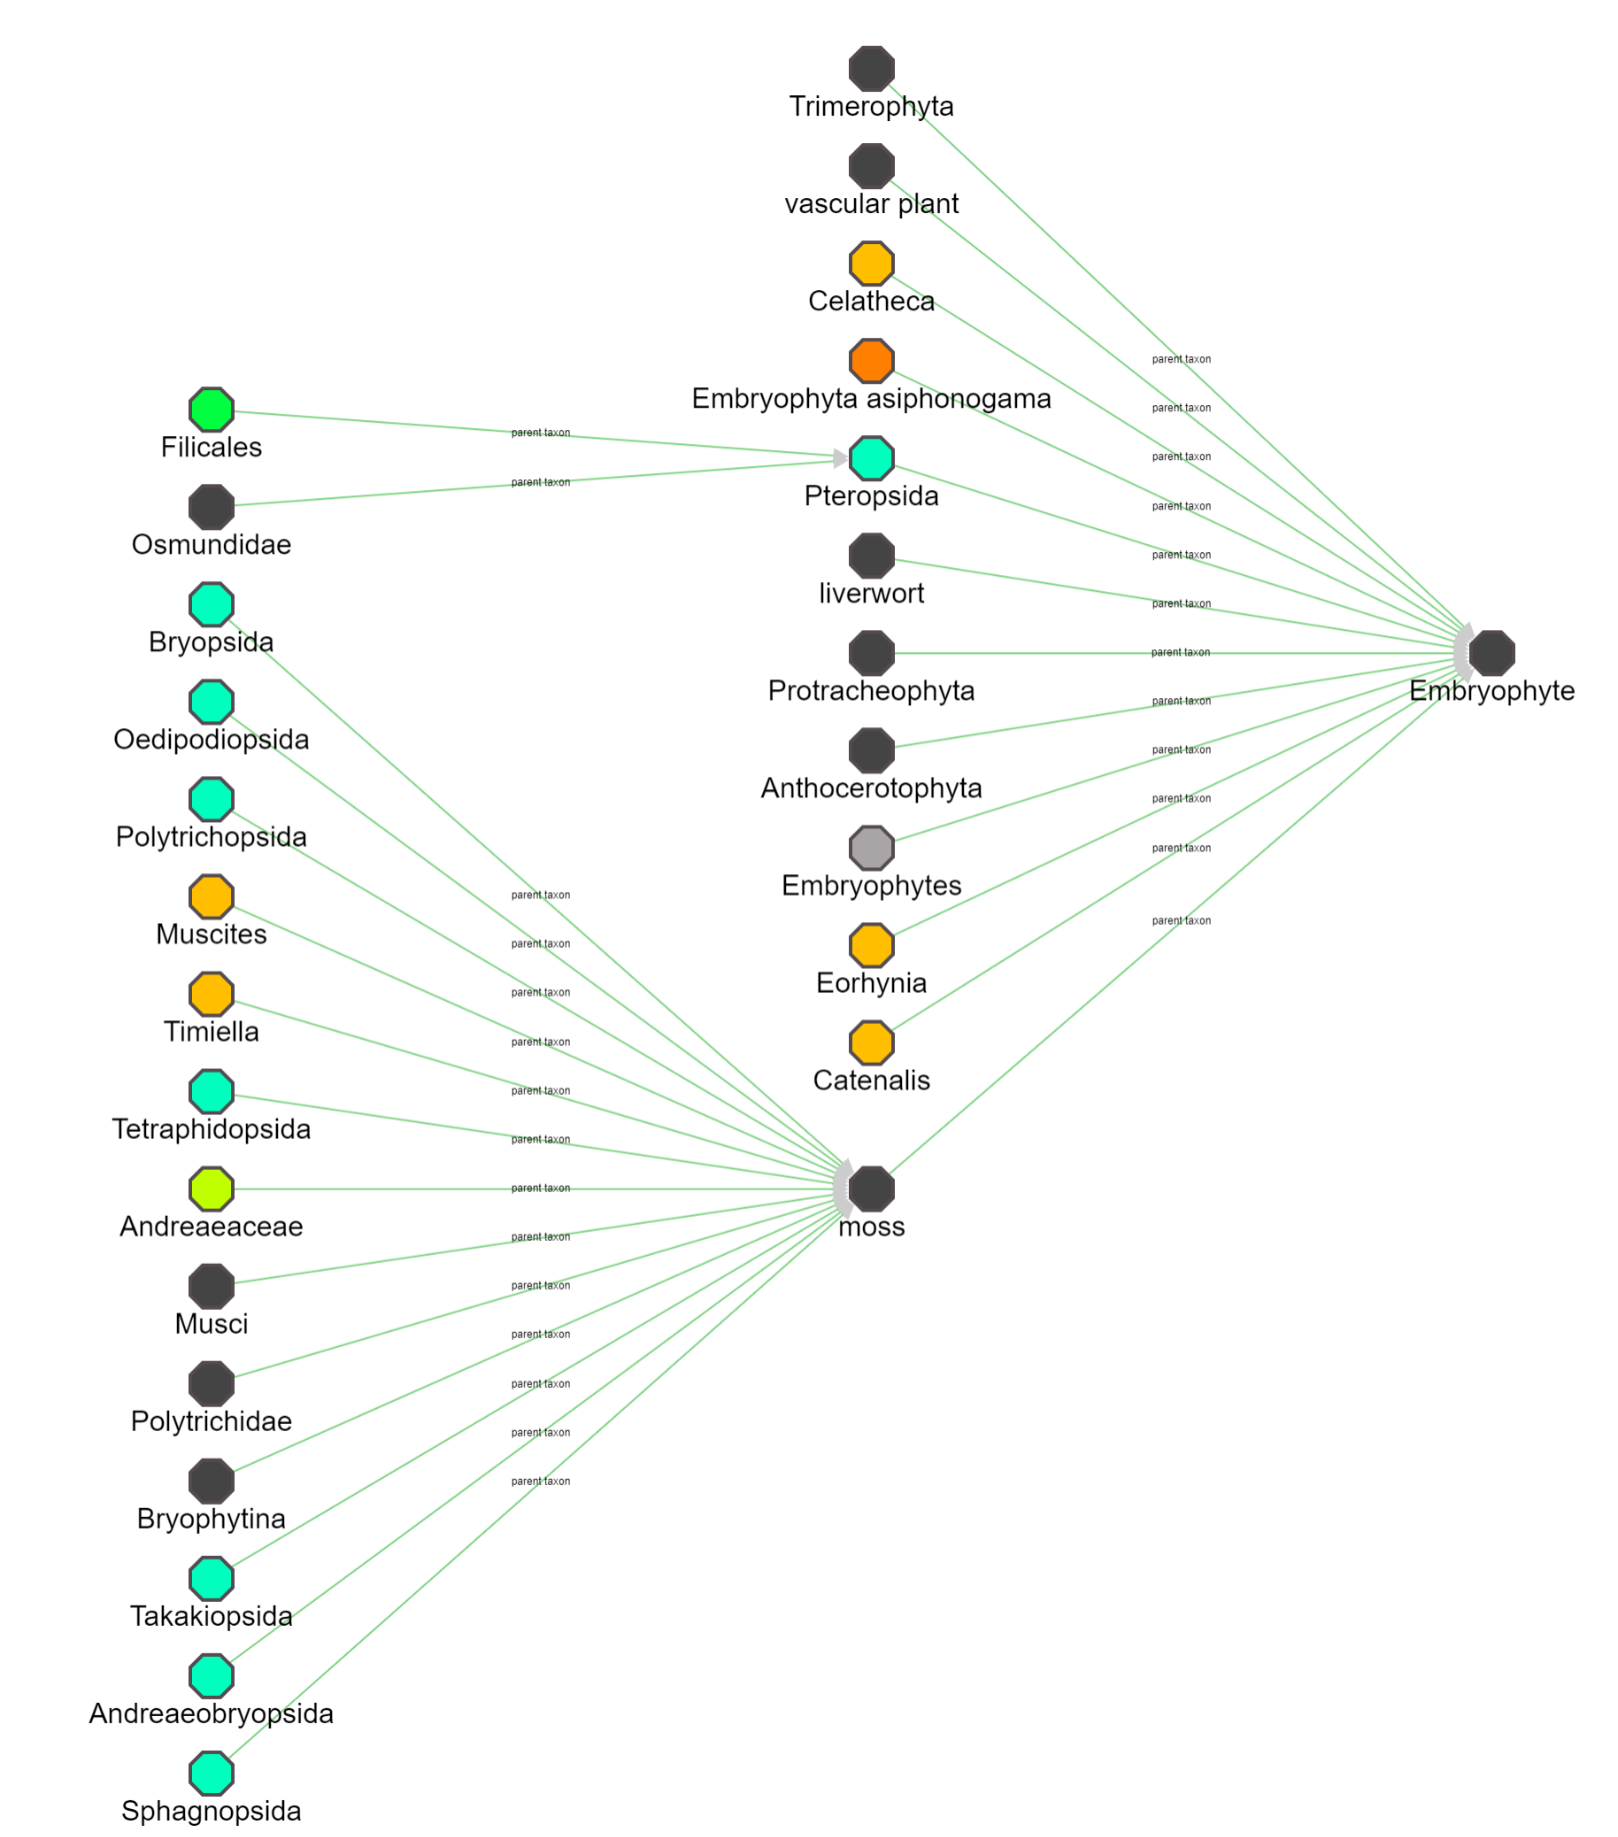
\includegraphics[width=0.5\textwidth]{media/sus-dagre.png}
    \end{figure}
    \item Stáhněte si aktuální graf do souboru, stránku aktualizujte a graf ze souboru opět načtěte.
    \item Nechte si zobrazit ze všech vrcholů jen ty, co mají třídu \uv{genus} (tedy chceme ty taxony, jež reprezentují rod).
    \item Odstraňte z grafu libovolný vrchol.
\end{enumerate}

\subsection{Výsledky testování SUS}

\todo{Zde budou zpracované otázky a výsledné skóre. Možná nějaké tabulky atp.}

\section{Výsledky obecných otázek}
V rámci testování SUS byli respondenti navíc dotázáni, jaké části aplikace pro ně byly uživatelsky nepřívětivé a čemu neporozumněli. Výsledky jsou sepsány v následujícím seznamu.

\begin{itemize}
    \item Tlačítka v pravém dolním rohu grafové oblasti sloužící na obsluhu grafu (layoutování, zobrazení celého grafu, kompaktní mód) nejsou popsány a respondent odpověděl, že měl problém zjistit, co dělají.

    Tlačítkům bude vhodné přidat tooltipy vysvětlující jejich funkce obdobně, jak je tomu v jiných částech aplikace.
    \item Respondent nepochopil uživatelské rozhraní pro výběr layoutu. Neuvědomil si, že jednotlivé karty odpovídají konkrétním layoutům a vždy je aktivní pouze jeden layout. Měnil nastavení jiného layoutu, než toho, který byl aktivní.

    Zvážit kompletní změnu uživatelského rozhraní, které uživatele nutí nejprve zvolit layout a poté měnit jeho natavení.
\end{itemize}

\bigskip

Úkoly popsané v rámci SUS průzkumu sloužily také jako určitá forma uživatelského testování aplikace. I když nebylo jasně definováno, jak by aplikace měla na konkrétní úkoly reagovat, můžeme předpokládat, že úkoly proběhly úspěšně, neboť je všichni z respondentů dokončili. Měřením code coverage bylo zjištěno, že provedením všech úkolů bylo pokryto 77\% kódu, tedy většina aplikace byla těmito úkoly úspěšně otestována. \uv{Provedením úkolů} je myšlena nejjednodušší cesta, jak daný úkol v aplikaci provést.

Měření bylo prováděno s pomocí IDE WebStorm\footnote{\url{https://www.jetbrains.com/webstorm/}} od JetBrains pod prohlížečem Google Chrome. Code coverage se měří ze řádků které byly v rámci aplikace spuštěny, přičemž se do výpočtu podílu nezahrnují komentáře, prázdné řádky a definice rozhraní, které se do JavaScriptu nepřekládají.
\chapter*{Závěr}
\addcontentsline{toc}{chapter}{Závěr}
V rámci této práce byla dle zadaných požadavků navržena, implementována a otestována webová aplikace pro procházení a vizualizaci dat z grafových databází. To, jak jsou data zobrazena a jakým způsobem je lze procházet popisuje konfigurace.

Uživatel si může do aplikace přidat vrcholy reprezentující existující entity a ty může expandovat a rozšiřovat tak graf o nové vrcholy. Aplikace poskytuje uživateli dodatečné informace o vrcholech, obarvuje je podle jejich typu, umožňuje filtrovat graf a podporuje několik layoutů, jak může být graf zobrazen. Pro snazší práci lze vrcholy seskupovat do skupin, a je možné si vrcholy zobrazit tak, aby je bylo snadné procházet po jejich sousedech.

\section{Možnosti vylepšení}
Tato kapitola rozebírá možné způsoby, jak aplikaci rozšířit do budoucna a možnou implementaci, jak tyto rozšíření provést.

\subsection*{Rozhraní mezi serverem a klientem}
Aktuálně je rozhraní navrženo tak, že serveru lze posílat požadavky samostatně. Toto řešení je nicméně nevyhovující v případě, kdy bude klient vyžadovat odpovědi na více požadavků současně. Budou-li poslány v jedné zprávě, kromě snížení komunikace mezi serverem a klientem bude moci server optimalizovat dotazy na datové zdroje. Kupříkladu dvě expanze lze teoreticky spojit do jednoho SPARQL dotazu.

Server také může posílat data, o která klient nežádal, v případě, že se bude domnívat, že je klient může požadovat. Například když klient požádá o \texttt{view-sets}, může server rovnou poslat \texttt{preview} na výchozí pohled, neboť o něj bude klient zřejmě žádat.

\subsection*{Cachování}
Problém cachování již v této práci rozebírán byl. S každým požadavkem klienta se server dotazuje datových zdrojů. Tato operace je časově náročná a zbytečně dochází k vytěžování datových zdrojů.

Kupříkladu SPARQL endpoint Wikidat má omezení na počet požadavků a při vysoké aktivitě klienta může server dostat IP ban.

Možnosti cachování jsou následující:
\begin{itemize}
    \item Cachovat výsledky jednotlivých dotazů. Například budou cachována data expanze pro každý vrchol kompletně zvlášť. Toto řešení je jednoduché, nicméně náročné na paměť, neboť jednotlivé vrcholy budou uložené několikrát.
    \item Cachovat malé bloky a ty pak sestavovat. V případě s expanzí bude uložen pouze seznam IRI vrcholů a data k vrcholům budou uložená samostatně. Tak dojde k omezení všech redundantních informací. U každého bloku bude uložen čas stažení, který bude kontrolován a v případě příliš starého výsledku se cache zahodí.
    \item Cachovat kompletní graf. Místo ukládání dat, která jsou výsledky jednotlivých dotazů, stáhneme část grafu a dotazy nad tímto grafem budou provedeny lokálně. Tímto jsme schopni z cache získat i taková data, na která se dotazujeme poprvé.
\end{itemize}

\subsection*{Detail}
Detail zobrazuje podrobné informace o vrcholu, které získá z různých literálů. Aktuálně je ignorován typ těchto literálů, je tedy možné s ním pracovat a na základě tohoto typu pak data zpracovávat. Kromě jednoduchých typů jako jsou čísla, můžeme zpracovávat například telefonní čísla, e-mailové adresy, nebo URL adresy.

Typem položky detailu může být i vrchol, přes který se pak bude moci uživatel dostat na skutečný vrchol v grafu. Tento vztah pak nahrazuje klasickou hranu v grafu a dá se použít tam, kde je podle autora konfigurace nevhodné, aby byly vrcholy spojené skutečnou hranou.

Detail je možné rozšířit i tak, aby neobsahoval jen skalární hodnoty, ale i pole a objekty. Toto opět nahrazuje klasický grafový přístup, kdy místo několika vrcholů (literálů) vypíšeme seznam těchto hodnot v detailu.

\subsection*{Práce s daty v detailu}
V případě, že budeme mít typované položky detailu, nabízí se s těmito daty pracovat.

Jednou možností je zvolit množinu vrcholů a jejich data vykreslit do grafu (myšleno jako koláčový/sloupcový graf). Uveďme konkrétní příklad, opět s Karlem Čapkem. Necháme si vrchol expandovat a zobrazit si všechna jeho díla. Za předpokladu, že u každého vrcholu díla je položka \uv{rok publikace}, můžeme z těchto dat sestavit histogram a podívat se, v jakém období Karel Čapek psal a kdy byl vrchol jeho kariéry.

Pokročilejším grafem by pak mohlo být zanesení roku díla na osu $x$ a popularitu tohoto díla na osu $y$.

\subsection*{Textové procházení grafem}
Pro některé scénáře může být pro uživatele nepraktické si vrcholy zobrazovat v grafu a hledat jednotlivé vrcholy v něm. Někdy může být žádoucí tyto vrcholy do grafu vůbec nepřidávat. V takovém případě by bylo možné přejít na textové procházení grafem, kdy se jednotlivé expanze vypíšou jako seznam vrcholů a uživatel jimi bude moct procházet obdobně jak je tomu u webových stránek. Všechny tyto vrcholy by se implicitně v grafu nezobrazovaly (tedy by nebyly \texttt{mounted}) a až konečný vrchol by uživatel mohl převést do grafu.

\subsection*{Nástroj pro úpravu a návrh konfigurací}
Aktuálně jsou konfigurace definovány pomocí Turtle notace v RDF grafech. To bohužel znemožňuje snadné vytváření konfigurací běžnými uživateli. Nabízí se tedy vytvořit nástroj, který by tyto konfigurace vytvářel a ukládal je do úložiště konfigurací, aby nebylo potřebné je ukládat ručně.

\section{Aplikace}
\textit{Tato sekce obsahuje snímky z aplikace a velmi stručný návod na její obsluhu. Cílem této sekce není poskytnutí uživatelské dokumentace. Pouze popisuje její základní principy.}

Po spuštění aplikace je uživatel vyzván k výběru konfigurace. V tomto okně je také možné zadat IRI konfigurace a meta konfigurace ručně, nebo otevřít existující graf ze souboru. Jakmile je uživatelem vybrána konfigurace, je vyzván k výběru prvního vrcholu, který bude přidán do grafu. To je možné provést ze seznamu předdefinovaných vrcholů, nebo může použít vyhledávací pole.

Hlavní okno aplikace má uprostřed grafovou oblast. S tou je možné manipulovat pomocí myši, nebo červených tlačítek v pravém dolním rohu. Po kliknutí na vrchol, označení více vrcholů, nebo skupiny se zobrazí pravý boční panel s detailními informacemi. Levý panel se automaticky skrývá a obsahuje další akce, které je možné s grafem provést. V levém horním rohu se také nachází pole, přes které lze přidávat a vyhledávat vrcholy v grafu.

\begin{figure}[h]
    \centering
    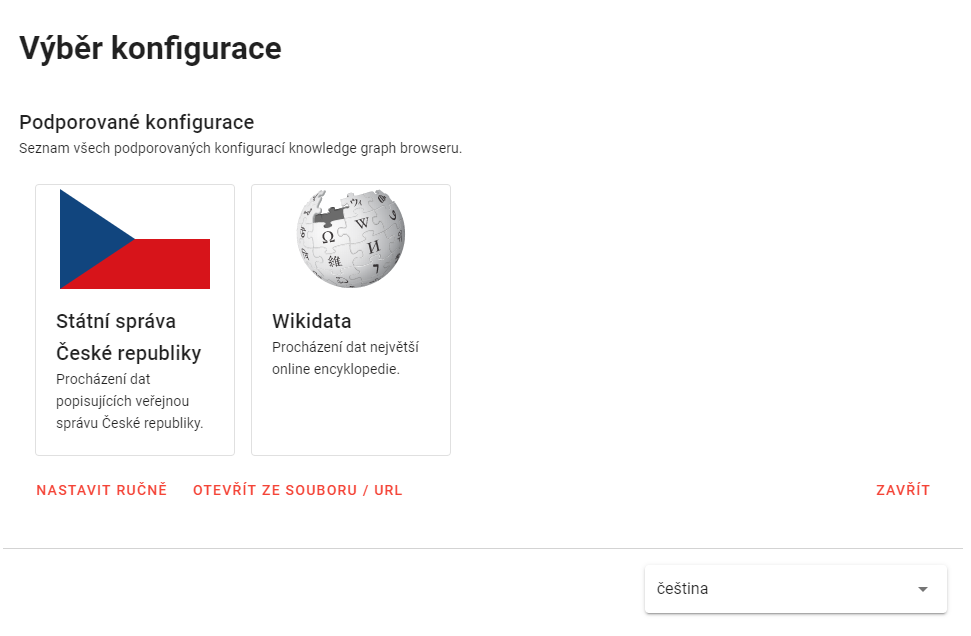
\includegraphics[width=\textwidth]{media/metaconfiguration.png}\\
    \caption{Úvodní obrazovka s výměrem mezi dvěma meta konfiguracemi. Je také možné ručně zadat IRI konfigurací nebo stáhnout graf ze souboru.}
\end{figure}

\newpage

\begin{figure}
    \centering
    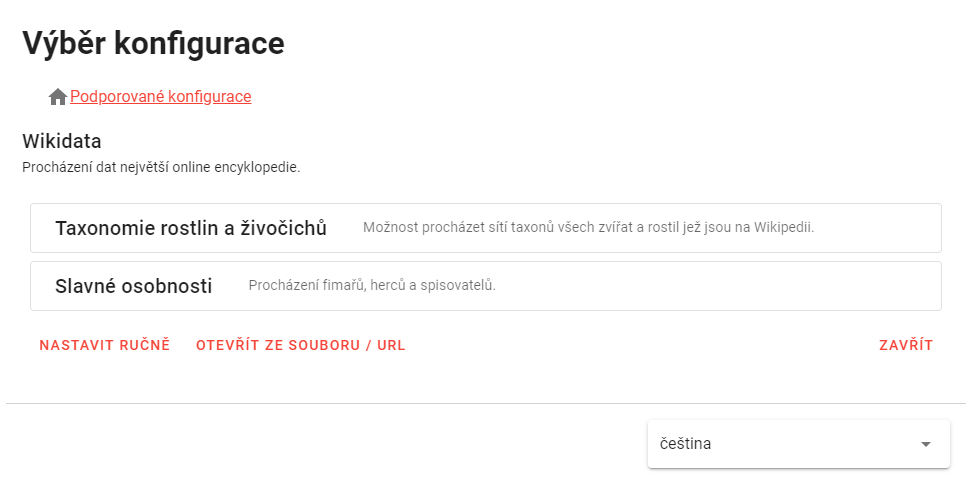
\includegraphics[width=\textwidth]{media/configuration.png}
    \caption{Obrazovka s výběrem konkrétních konfigurací v rámci Wikipedie (Wikidat).}
    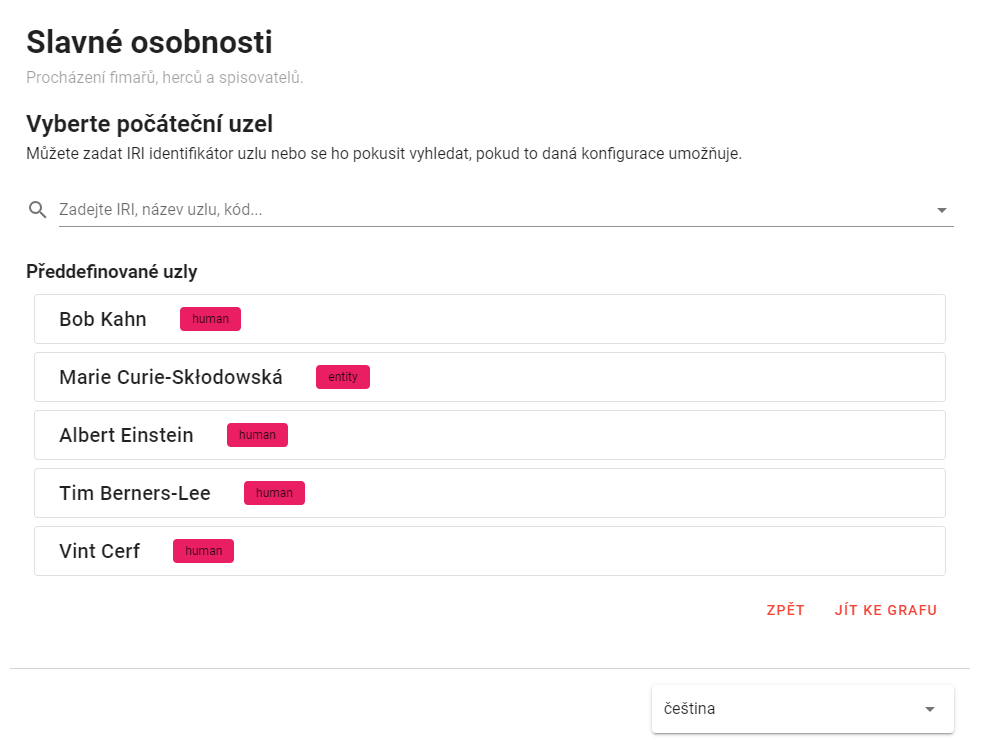
\includegraphics[width=\textwidth]{media/node-selection.png}
    \caption{Obrazovka s výběrem počátečního vrcholu. Ten je možné vybrat z předdefinovaných, nebo je možné použít vyhledávací pole.}
\end{figure}

\newpage

\begin{figure}
    \centering
    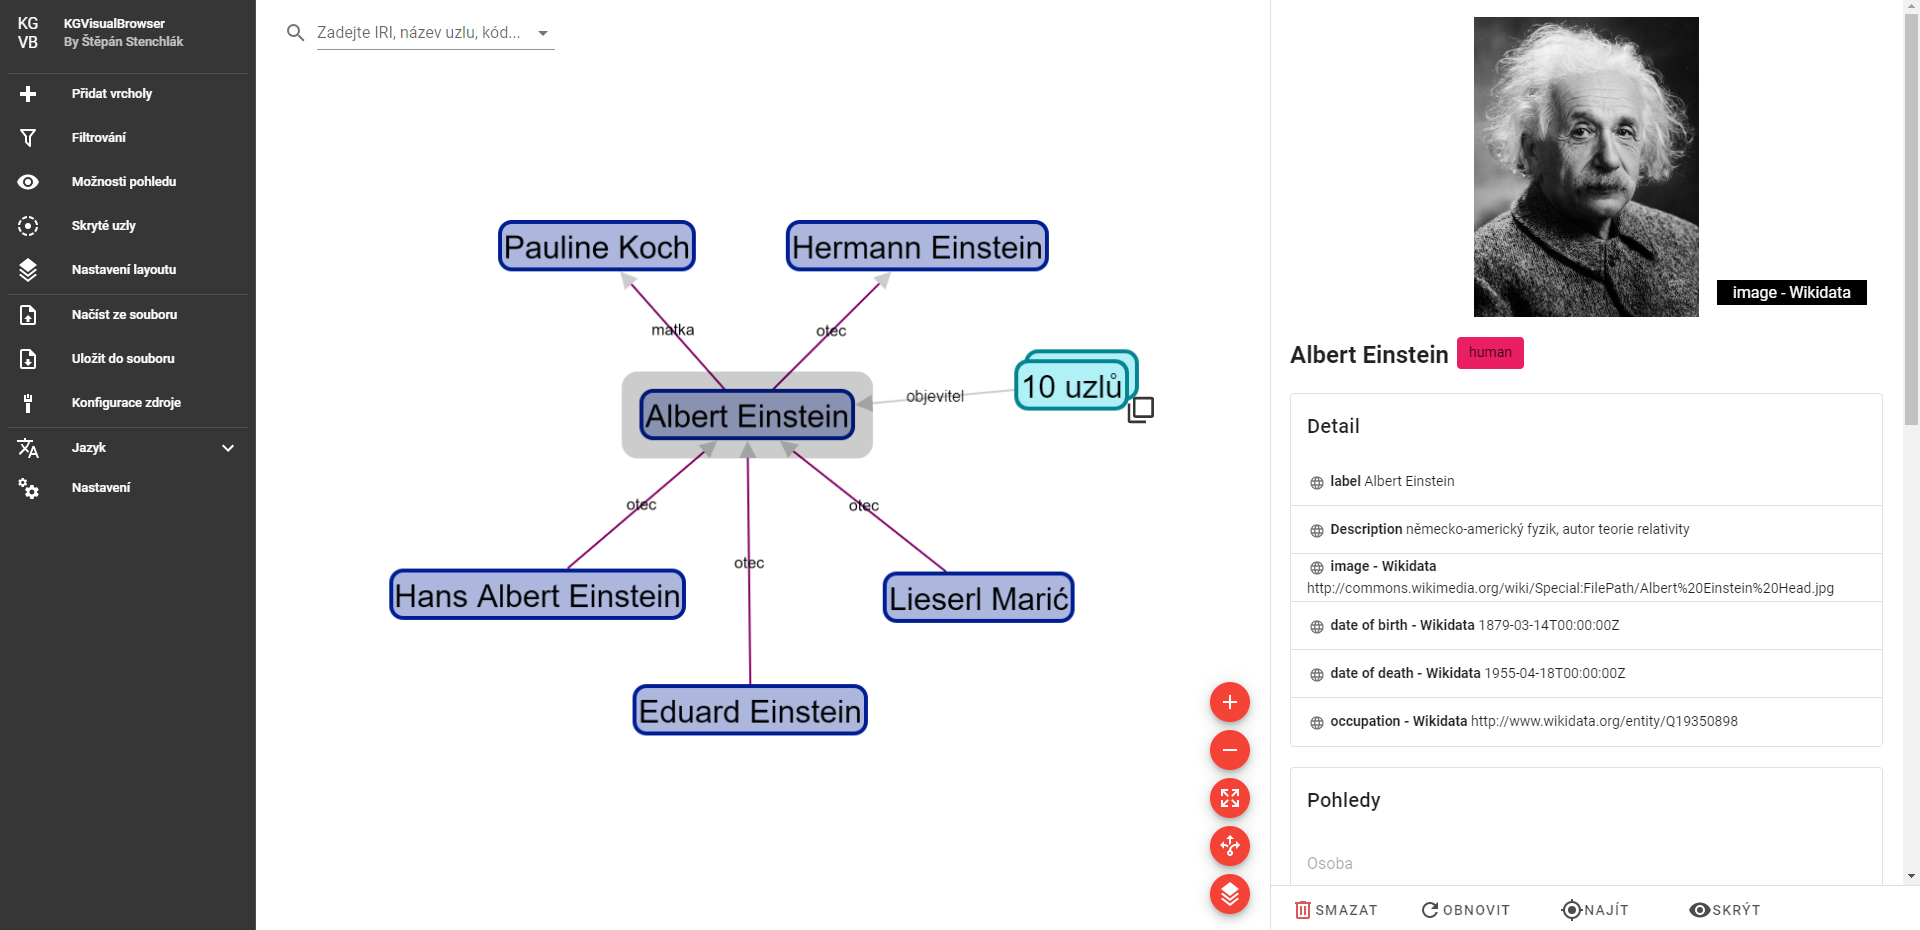
\includegraphics[width=\textwidth]{media/einstein.png}
    \caption{Hlavní okno aplikace s již načteným grafem a vybraným vrcholem. Levý panel je zde rozevřený.}
    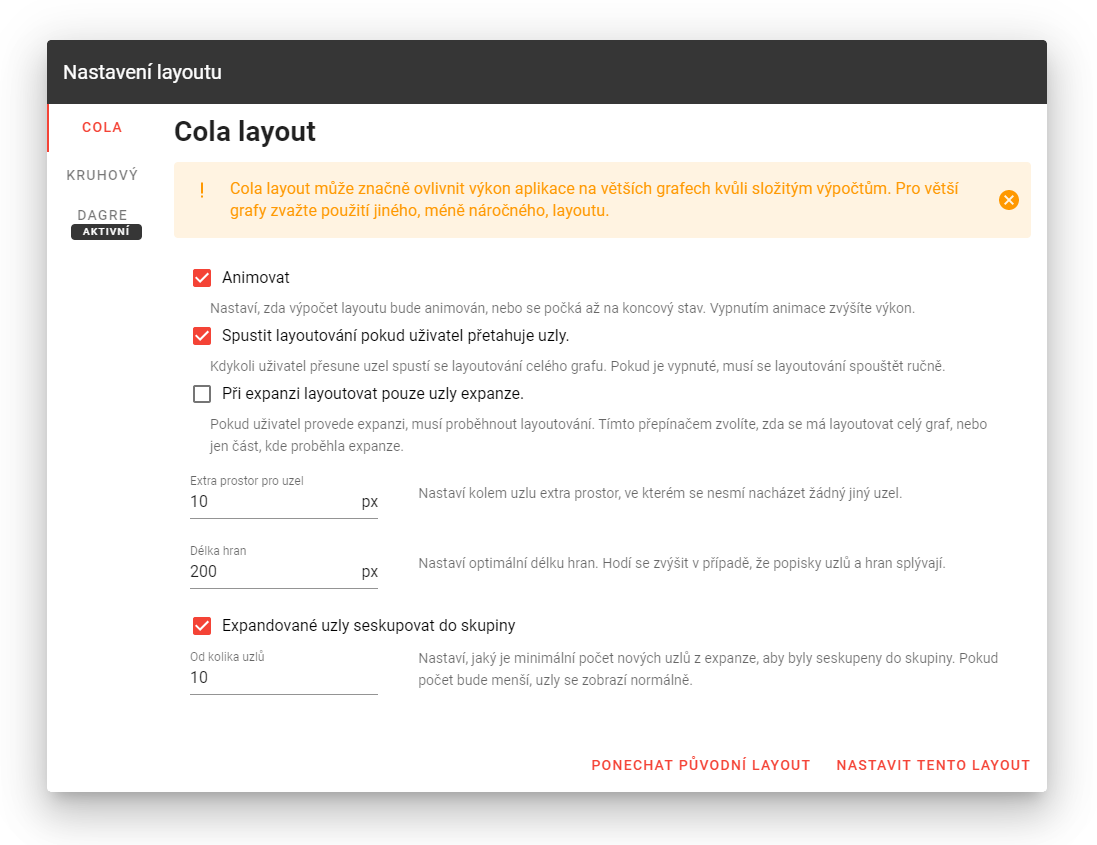
\includegraphics[width=\textwidth]{media/layout.png}
    \caption{Dialog pro výběr a nastavení layoutů.}
\end{figure}

%%% Seznam použité literatury
%%% Seznam použité literatury (bibliografie)
%%%
%%% Pro vytváření bibliografie používáme bibTeX. Ten zpracovává
%%% citace v textu (např. makro \cite{...}) a vyhledává k nim literaturu
%%% v souboru literatura.bib.
%%%
%%% Příkaz \bibliographystyle určuje, jakým stylem budou citovány odkazy
%%% v textu. V závorce je název zvoleného souboru .bst. Styly plainnat
%%% a unsrt jsou standardní součástí latexových distribucí. Styl czplainnat
%%% je dodáván s touto šablonou a bibTeX ho hledá v aktuálním adresáři.

\bibliographystyle{czplainnat}    %% Autor (rok) s českými spojkami
% \bibliographystyle{plainnat}    %% Autor (rok) s anglickými spojkami
% \bibliographystyle{unsrt}       %% [číslo]

\renewcommand{\bibname}{Seznam použité literatury}

%%% Vytvoření seznamu literatury. Pozor, pokud jste necitovali ani jednu
%%% položku, seznam se automaticky vynechá.

\bibliography{literatura}

%%% Kdybyste chtěli bibliografii vytvářet ručně (bez bibTeXu), lze to udělat
%%% následovně. V takovém případě se řiďte normou ISO 690 a zvyklostmi v oboru.

% \begin{thebibliography}{99}
%
% \bibitem{lamport94}
%   {\sc Lamport,} Leslie.
%   \emph{\LaTeX: A Document Preparation System}.
%   2. vydání.
%   Massachusetts: Addison Wesley, 1994.
%   ISBN 0-201-52983-1.
%
% \end{thebibliography}


%%% Obrázky v bakalářské práci
%%% (pokud jich je malé množství, obvykle není třeba seznam uvádět)
\listoffigures

%%% Tabulky v bakalářské práci (opět nemusí být nutné uvádět)
%%% U matematických prací může být lepší přemístit seznam tabulek na začátek práce.
\listoftables

%%% Použité zkratky v bakalářské práci (opět nemusí být nutné uvádět)
%%% U matematických prací může být lepší přemístit seznam zkratek na začátek práce.
\chapwithtoc{Seznam použitých zkratek}

%%% Přílohy k bakalářské práci, existují-li. Každá příloha musí být alespoň jednou
%%% odkazována z vlastního textu práce. Přílohy se číslují.
%%%
%%% Do tištěné verze se spíše hodí přílohy, které lze číst a prohlížet (dodatečné
%%% tabulky a grafy, různé textové doplňky, ukázky výstupů z počítačových programů,
%%% apod.). Do elektronické verze se hodí přílohy, které budou spíše používány
%%% v elektronické podobě než čteny (zdrojové kódy programů, datové soubory,
%%% interaktivní grafy apod.). Elektronické přílohy se nahrávají do SISu a lze
%%% je také do práce vložit na CD/DVD. Povolené formáty souborů specifikuje
%%% opatření rektora č. 72/2017.
\appendix
\chapter{Přílohy}

\section{První příloha}

\openright
\end{document}
